\documentclass[conference]{IEEEtran}
\IEEEoverridecommandlockouts
\usepackage{cite}
\usepackage{amsmath,amssymb,amsfonts}
\usepackage{algorithmic}
\usepackage{graphicx}
\usepackage{textcomp}
\usepackage{xcolor}
\usepackage{booktabs}
\usepackage{url}
\usepackage{multirow}
\usepackage{subcaption}
\def\BibTeX{{\rm B\kern-.05em{\sc i\kern-.025em b}\kern-.08em
    T\kern-.1667em\lower.7ex\hbox{E}\kern-.125emX}}
\begin{document}

\title{EV Charging Station Suitability Analysis Using Multispectral OSM Classification and Machine Learning-Based Site Prediction}

\author{\IEEEauthorblockN{1\textsuperscript{st} Author Name}
\IEEEauthorblockA{\textit{Dept. of Computer Science and Engineering} \\
\textit{Indian Institute of Technology (BHU)}\\
Varanasi, India \\
author1@iitbhu.ac.in}
\and
\IEEEauthorblockN{2\textsuperscript{nd} Author Name}
\IEEEauthorblockA{\textit{Dept. of Computer Science and Engineering} \\
\textit{Indian Institute of Technology (BHU)}\\
Varanasi, India \\
author2@iitbhu.ac.in}
}

\maketitle

\begin{abstract}
Strategic placement of Electric Vehicle (EV) charging stations is critical for accelerating EV adoption in India. This paper presents an end-to-end, open-data-driven pipeline for identifying optimal EV charging locations using OpenStreetMap (OSM) data. The system operates in two phases: (1) a multispectral classification engine that parses raw OSM files to produce colour-coded spatial maps categorising roads, buildings, and land use into over 30 fine-grained classes, along with a heuristic suitability heatmap and 3D extruded visualisation; and (2) a supervised Random Forest classifier trained on real EV station coordinates across Indian cities via the Overpass API, using a 23-dimensional spatial feature vector extracted from the surrounding urban fabric. The pipeline is validated on three geographically diverse sites: BHU Campus (Varanasi), IIT Delhi (New Delhi), and Majestic Area (Bangalore). The ML model achieves a mean cross-validated ROC-AUC of 0.678 and successfully differentiates dense urban zones (Bangalore Majestic: top score 0.811, all HIGH priority) from semi-rural university campuses (BHU: scores 0.56--0.59, all MEDIUM priority). Feature importance analysis reveals that POI density, amenity count, and restaurant/cafe presence are the strongest predictors of real-world EV station placement. The entire system is open-source, lightweight (approximately 1,800 lines of Python), and requires no proprietary software, GIS licenses, or GPU hardware.
\end{abstract}

\begin{IEEEkeywords}
electric vehicle, charging station, OpenStreetMap, random forest, spatial analysis, multispectral classification, site prediction, GIS
\end{IEEEkeywords}

\section{Introduction}

\subsection{Background and Motivation}

India has witnessed a rapid surge in Electric Vehicle (EV) adoption, driven by government policies such as the FAME-II scheme~\cite{b6}, rising fuel prices, and growing environmental awareness. The Indian EV market is projected to reach 10 million annual sales by 2030~\cite{b1}. However, the growth of EVs is fundamentally constrained by the availability of charging infrastructure. Unlike conventional fuel stations, EV chargers must be strategically placed to minimise range anxiety, maximise utilisation, and ensure equitable access across urban and semi-urban spaces.

Current approaches to EV station placement in India are largely ad hoc---driven by land availability or commercial partnerships rather than data-driven spatial analysis. This leads to clustering of chargers in some areas while leaving vast regions underserved. University campuses, in particular, represent ideal testbeds for EV charging infrastructure due to their well-defined boundaries, diverse building typologies (hostels, academic blocks, hospitals, sports complexes), multi-modal road networks, and high population density of early EV adopters.

\subsection{Problem Statement}

Given an arbitrary geographic area represented as an OpenStreetMap (OSM) file, the objectives are:
\begin{enumerate}
\item Classify every spatial feature (roads, buildings, land use, water bodies) into fine-grained categories using a multispectral colour-coding scheme derived from OSM tags.
\item Score each location for EV charging suitability using a rule-based heuristic weighted model.
\item Train a supervised Machine Learning classifier on real-world EV charging station locations across Indian cities.
\item Predict optimal EV charging station placement on any new, unseen map using the trained ML model.
\item Visualise results through 2D maps, 3D extruded models, heatmaps, and ranked JSON reports.
\end{enumerate}

\subsection{Use Cases}

The system serves multiple stakeholders: urban planners can rapidly assess any area's readiness for EV infrastructure using open data; municipal bodies can prioritise budget allocation for charger installation using data-backed rankings; campus administrators can plan internal EV charging networks for universities, tech parks, and hospitals; researchers can study spatial patterns of existing EV infrastructure; and EV startups can identify high-demand, underserved areas for new station deployment.

\subsection{Scope}

The prototype is built and demonstrated on three geographically diverse sites in India: (1) BHU Campus, Varanasi---a 1,300-acre campus with 15,162 OSM nodes and 1,686 ways; (2) IIT Delhi Campus, New Delhi---a compact urban campus; and (3) Majestic Area, Bangalore---a dense urban commercial zone and high-density transit hub.


\section{Literature Review}

\subsection{EV Charging Station Placement}

Significant research exists on optimal EV charger placement using operations research and GIS-based methods. Flow-based models such as the Flow-Refueling Location Model (FRLM)~\cite{b7} optimise station placement along traffic corridors to maximise intercepted vehicle flows. GIS suitability analysis employs Multi-Criteria Decision Analysis (MCDA) with weighted overlay of factors like road proximity, land use, population density, and grid connectivity. More recently, Machine Learning approaches apply Random Forests, gradient boosting, and neural networks to predict optimal locations from urban feature vectors, learning patterns from existing successful deployments.

\subsection{OpenStreetMap as a Data Source}

OpenStreetMap (OSM) is the world's largest crowdsourced geospatial database, containing over 10 billion data points~\cite{b2}. OSM data is available under the Open Database License (ODbL) and can be exported for any region in XML format (\texttt{.osm}). Key advantages include: free, open-access, and globally available data; a rich tagging system for roads, buildings, amenities, and land use; real-time queryability via the Overpass API~\cite{b3}; and regular community-driven updates. These properties make OSM an ideal data source for scalable spatial analysis without the cost barriers of proprietary GIS datasets.

\subsection{Random Forest for Spatial Prediction}

Random Forest~\cite{b5} is an ensemble learning method that constructs multiple decision trees during training and outputs the class that is the mode of the individual trees. It is particularly well-suited for spatial prediction because it handles mixed feature types (binary, count, continuous) natively, provides built-in feature importance via Mean Decrease Impurity (MDI), is robust to overfitting with proper hyperparameter tuning, and does not require feature normalisation or scaling. These properties make it preferable to simpler classifiers for heterogeneous geospatial feature vectors.


\section{System Architecture}

\subsection{High-Level Architecture}

The system is organised as a two-phase pipeline controlled by a unified entry point (\texttt{main.py}). Phase~1 performs multispectral OSM classification entirely offline, producing five output artefacts. Phase~2 handles ML-based EV station prediction, with optional training via the Overpass API.

The data flow proceeds as follows: a raw \texttt{.osm} file is parsed to extract nodes and ways, which are then classified into categories. Three parallel visualisation outputs are generated (2D multispectral map, EV suitability heatmap, and 3D extruded map), along with a legend panel and a JSON report. The ML prediction phase then produces an additional prediction map, feature importance chart, and ML-specific JSON report.

\subsection{Project Structure}

\begin{table}[htbp]
\caption{Project Files and Their Roles}
\begin{center}
\begin{tabular}{|l|l|}
\hline
\textbf{File} & \textbf{Role} \\
\hline
\texttt{main.py} & Unified pipeline runner (CLI entry) \\
\hline
\texttt{ev\_campus\_analyzer.py} & Phase 1: Multispectral OSM (928 LOC) \\
\hline
\texttt{ev\_ml\_predictor.py} & Phase 2: ML prediction (888 LOC) \\
\hline
\texttt{identity.py} & Utility: inject EV nodes into OSM \\
\hline
\texttt{requirements.txt} & Python dependencies \\
\hline
\texttt{map.osm} & BHU campus OSM data (3.4\,MB) \\
\hline
\texttt{ev-charging-stations-india.csv} & India EV station dataset (228\,KB) \\
\hline
\end{tabular}
\label{tab:project}
\end{center}
\end{table}

\subsection{Technology Stack}

\begin{table}[htbp]
\caption{Technology Stack and Dependencies}
\begin{center}
\begin{tabular}{|l|l|l|}
\hline
\textbf{Component} & \textbf{Library} & \textbf{Purpose} \\
\hline
Language & Python 3.8+ & Core implementation \\
\hline
XML Parsing & xml.etree & OSM file parsing \\
\hline
Numerical & NumPy & Array ops, Gaussian kernels \\
\hline
Visualisation & Matplotlib & 2D maps, 3D, heatmaps \\
\hline
ML Framework & scikit-learn & Random Forest, CV \\
\hline
Data Handling & pandas & CSV I/O, feature matrices \\
\hline
Persistence & joblib & Save/load trained model \\
\hline
API Access & requests & Overpass API queries \\
\hline
Fast XML & lxml (optional) & Accelerated large file parsing \\
\hline
\end{tabular}
\label{tab:tech}
\end{center}
\end{table}


\section{Phase 1: Multispectral OSM Classification}

\subsection{Overview}

Phase~1 ingests a raw \texttt{.osm} file and produces five output artefacts: a 2D classification map, an EV suitability heatmap, a 3D extruded map, a colour legend with statistics, and a JSON report containing ranked candidate zones. The entire phase operates offline and requires no internet access.

\subsection{OSM Parsing}

The \texttt{OSMParser} class reads the XML structure, extracting three types of elements: nodes (latitude, longitude, and optional tags for each point), ways (ordered sequences of node references plus key-value tags describing the feature), and bounds (the geographic bounding box defined by \texttt{minlat}, \texttt{maxlat}, \texttt{minlon}, \texttt{maxlon}). For the BHU campus, 15,162 nodes and 1,686 ways were parsed from a 3.4\,MB OSM file.

\subsection{Feature Classification}

The \texttt{classify\_way()} function is the classification engine. It inspects OSM tags in a priority order to assign each way to exactly one of over 30 categories.

\subsubsection{Road Classification}

Road width is not directly available in OSM for most ways. Instead, width is inferred from the \texttt{highway=*} tag hierarchy, as shown in Table~\ref{tab:roads}.

\begin{table}[htbp]
\caption{Road Classification by OSM Highway Type}
\begin{center}
\begin{tabular}{|l|l|l|}
\hline
\textbf{OSM Tag} & \textbf{Category} & \textbf{Width} \\
\hline
\texttt{primary} & Primary Road & $>$12\,m \\
\hline
\texttt{secondary} & Secondary Road & 8--12\,m \\
\hline
\texttt{tertiary} & Tertiary Road & 6--8\,m \\
\hline
\texttt{residential} & Residential Road & $<$6\,m \\
\hline
\texttt{service} & Service Road / Alley & narrow \\
\hline
\texttt{footway} & Footway / Pedestrian & --- \\
\hline
\texttt{cycleway} & Cycleway & --- \\
\hline
\texttt{path/track} & Unpaved Path & --- \\
\hline
\end{tabular}
\label{tab:roads}
\end{center}
\end{table}

\subsubsection{Building Classification}

Buildings are classified into 11 functional categories using a combination of direct OSM tags (\texttt{building=*}, \texttt{amenity=*}, \texttt{healthcare=*}, \texttt{leisure=*}, \texttt{tourism=*}) and name-based keyword matching. Over 80 keywords (e.g., ``hostel'', ``hospital'', ``canteen'', ``mandir'') are matched against the \texttt{name=*} tag for buildings that lack explicit functional tags. Categories include: Academic/Lab, Hostel, Residential, Hospital, Temple, Sports, Library/Museum, Admin/Office, Canteen, Gate, and Generic (unclassified).

\subsubsection{Land Use and Natural Features}

Nine land-use categories are distinguished: Forest, Grassland, Garden/Park, Farmland, Barren/Open, Recreation, Water Body, Wetland, and Aquaculture. Each category is assigned a unique colour for the multispectral map output.

\subsection{EV Suitability Scoring (Heuristic)}

Each OSM way is assigned a suitability score in $[0, 1]$ via a weighted additive model. The scoring criteria and weights are shown in Table~\ref{tab:ev_score}.

\begin{table}[htbp]
\caption{Heuristic EV Suitability Scoring Weights}
\begin{center}
\begin{tabular}{|l|r|}
\hline
\textbf{Criterion} & \textbf{Weight} \\
\hline
Primary / secondary road access & $+0.40$ \\
\hline
Parking area & $+0.35$ \\
\hline
University / college amenity & $+0.30$ \\
\hline
Hospital / library nearby & $+0.25$ \\
\hline
Conference / community centre & $+0.22$ \\
\hline
Education land use & $+0.20$ \\
\hline
Name keywords (gate, parking) & $+0.20$ \\
\hline
Restaurant / cafe (footfall proxy) & $+0.12$ \\
\hline
Recreation ground & $+0.12$ \\
\hline
Water body / waterway (penalty) & $-0.20$ to $-0.30$ \\
\hline
\end{tabular}
\label{tab:ev_score}
\end{center}
\end{table}

The scoring function serves two purposes: generating the suitability heatmap via Gaussian kernel density estimation on a $250 \times 250$ grid, and producing the ranked candidate zone list in the JSON report. Zones are classified into three priority tiers: HIGH ($\geq 0.55$) indicating strong candidate zones, MEDIUM ($0.40$--$0.54$) indicating moderate candidates, and LOW ($< 0.40$) indicating lower priority areas.

\subsection{3D Visualisation}

Buildings are extruded to pseudo-3D heights based on their functional category, as shown in Table~\ref{tab:heights}. When the OSM \texttt{height=*} tag is present, the actual height is used (capped at 0.12 relative units for visual clarity). Land-use patches are rendered as flat ground layers at near-zero elevations.

\begin{table}[htbp]
\caption{Default Extrusion Heights by Building Category}
\begin{center}
\begin{tabular}{|l|r|}
\hline
\textbf{Category} & \textbf{Relative Height} \\
\hline
Academic / Dept / Lab & 0.060 \\
\hline
Hospital / Medical & 0.050 \\
\hline
Temple / Place of Worship & 0.045 \\
\hline
Library / Museum & 0.042 \\
\hline
Hostel / Student Housing & 0.040 \\
\hline
Admin / Office & 0.038 \\
\hline
Sports / Pool & 0.035 \\
\hline
Residential (Staff) & 0.030 \\
\hline
Canteen / Cafe & 0.025 \\
\hline
Generic (Unclassified) & 0.020 \\
\hline
Gate / Entrance & 0.015 \\
\hline
\end{tabular}
\label{tab:heights}
\end{center}
\end{table}

\subsection{Phase 1 Outputs}

\begin{figure}[htbp]
\centerline{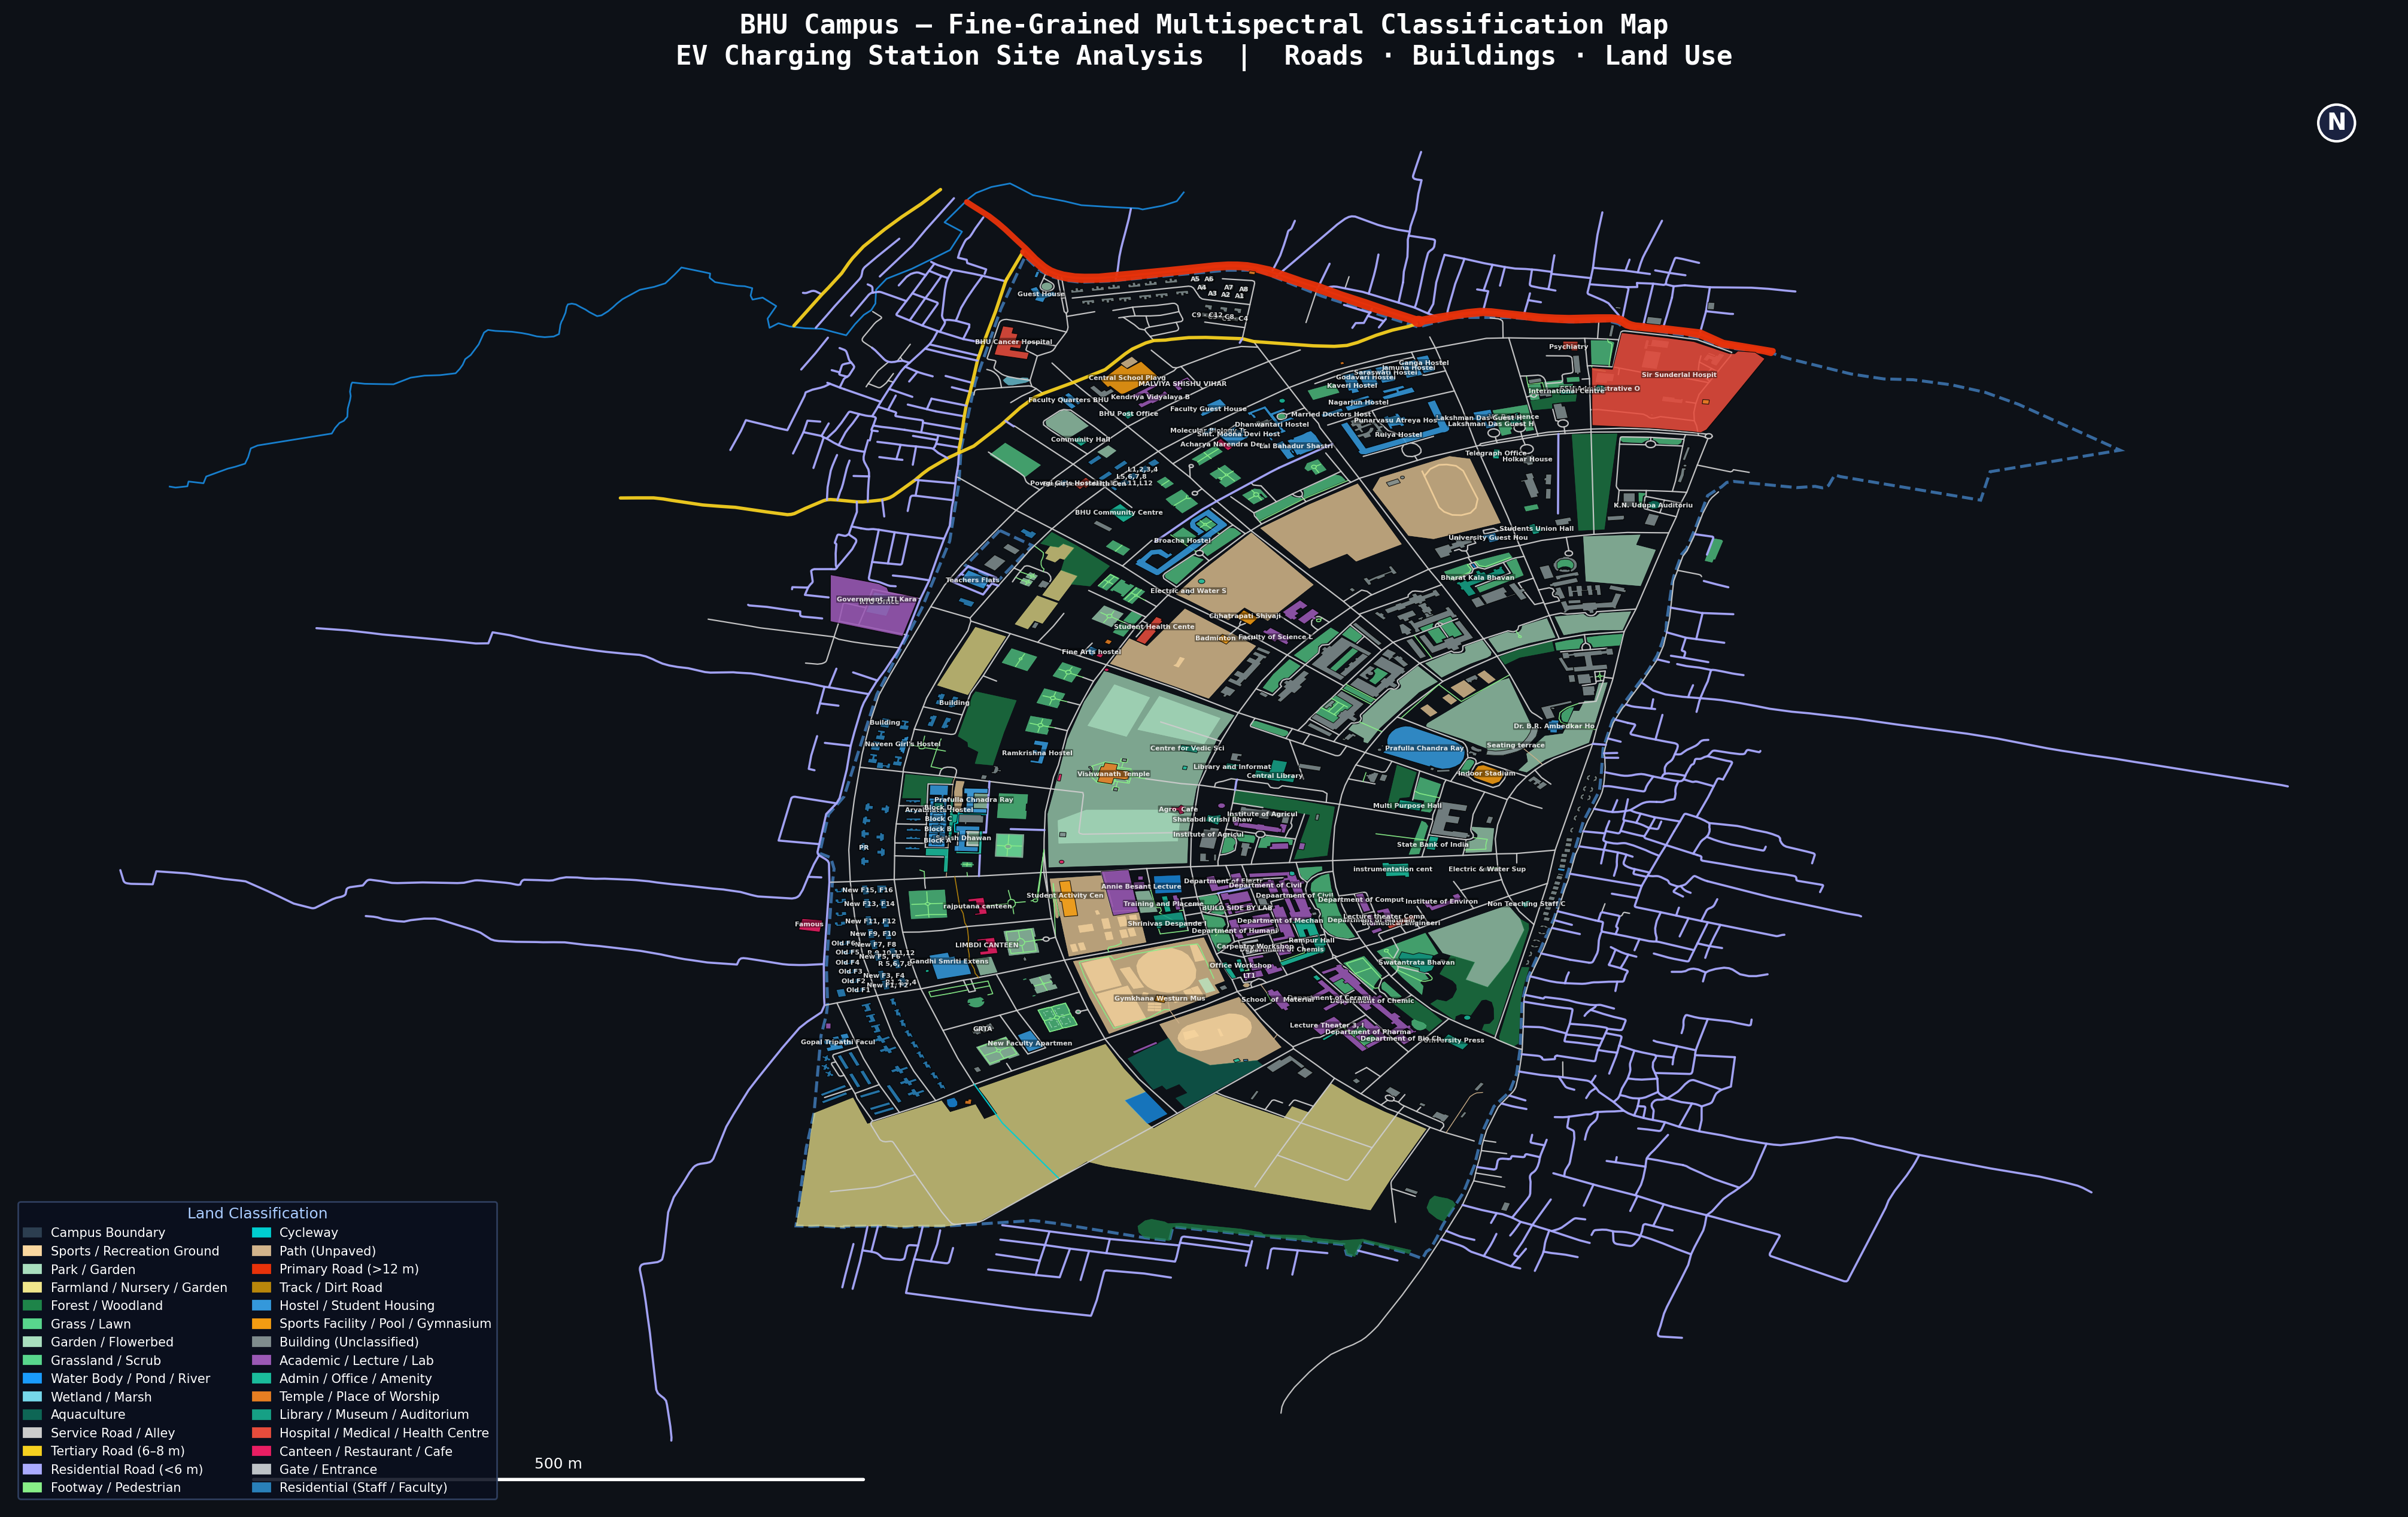
\includegraphics[width=0.48\textwidth]{figures/bhu_multispectral.png}}
\caption{2D Multispectral Classification Map for BHU Campus. Each feature is colour-coded by its functional category: roads by hierarchy, buildings by function, and land patches by type.}
\label{fig:bhu_multi}
\end{figure}

\begin{figure}[htbp]
\centerline{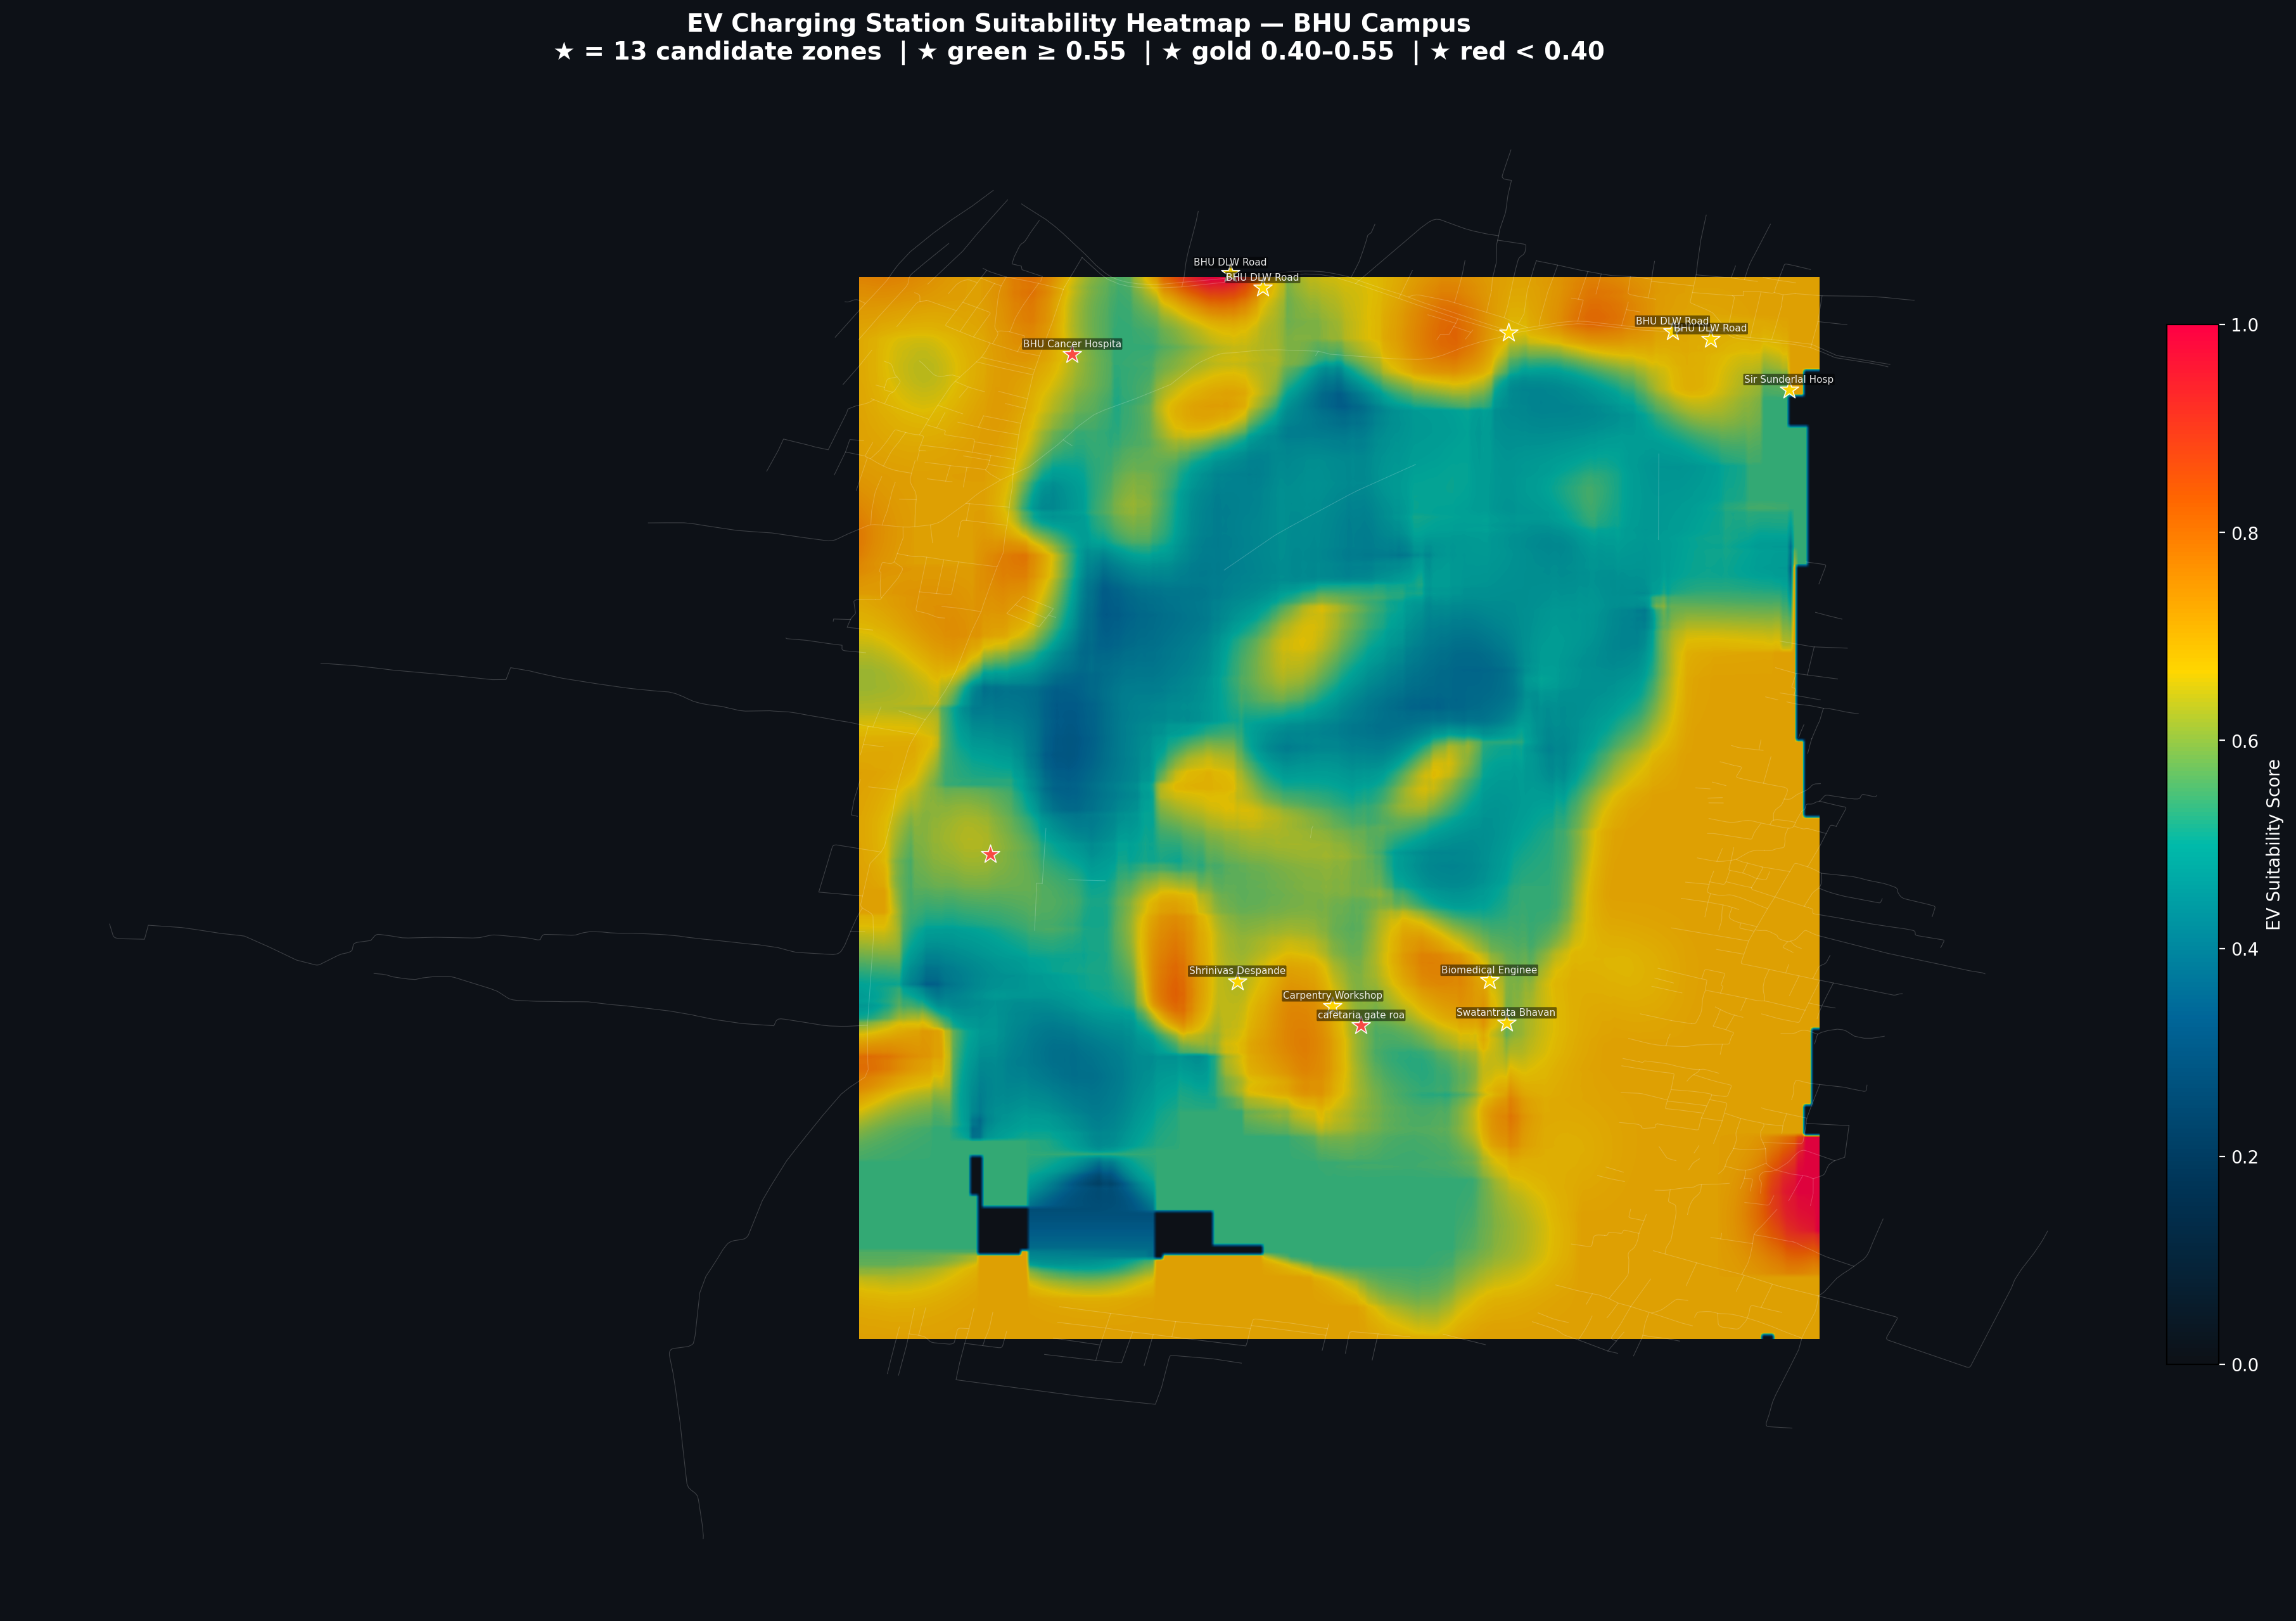
\includegraphics[width=0.45\textwidth]{figures/bhu_heatmap.png}}
\caption{EV Suitability Heatmap for BHU Campus. Star markers indicate the top candidate zones. The colour scale ranges from cool (low suitability) to warm (high suitability).}
\label{fig:bhu_heat}
\end{figure}

\begin{figure}[htbp]
\centerline{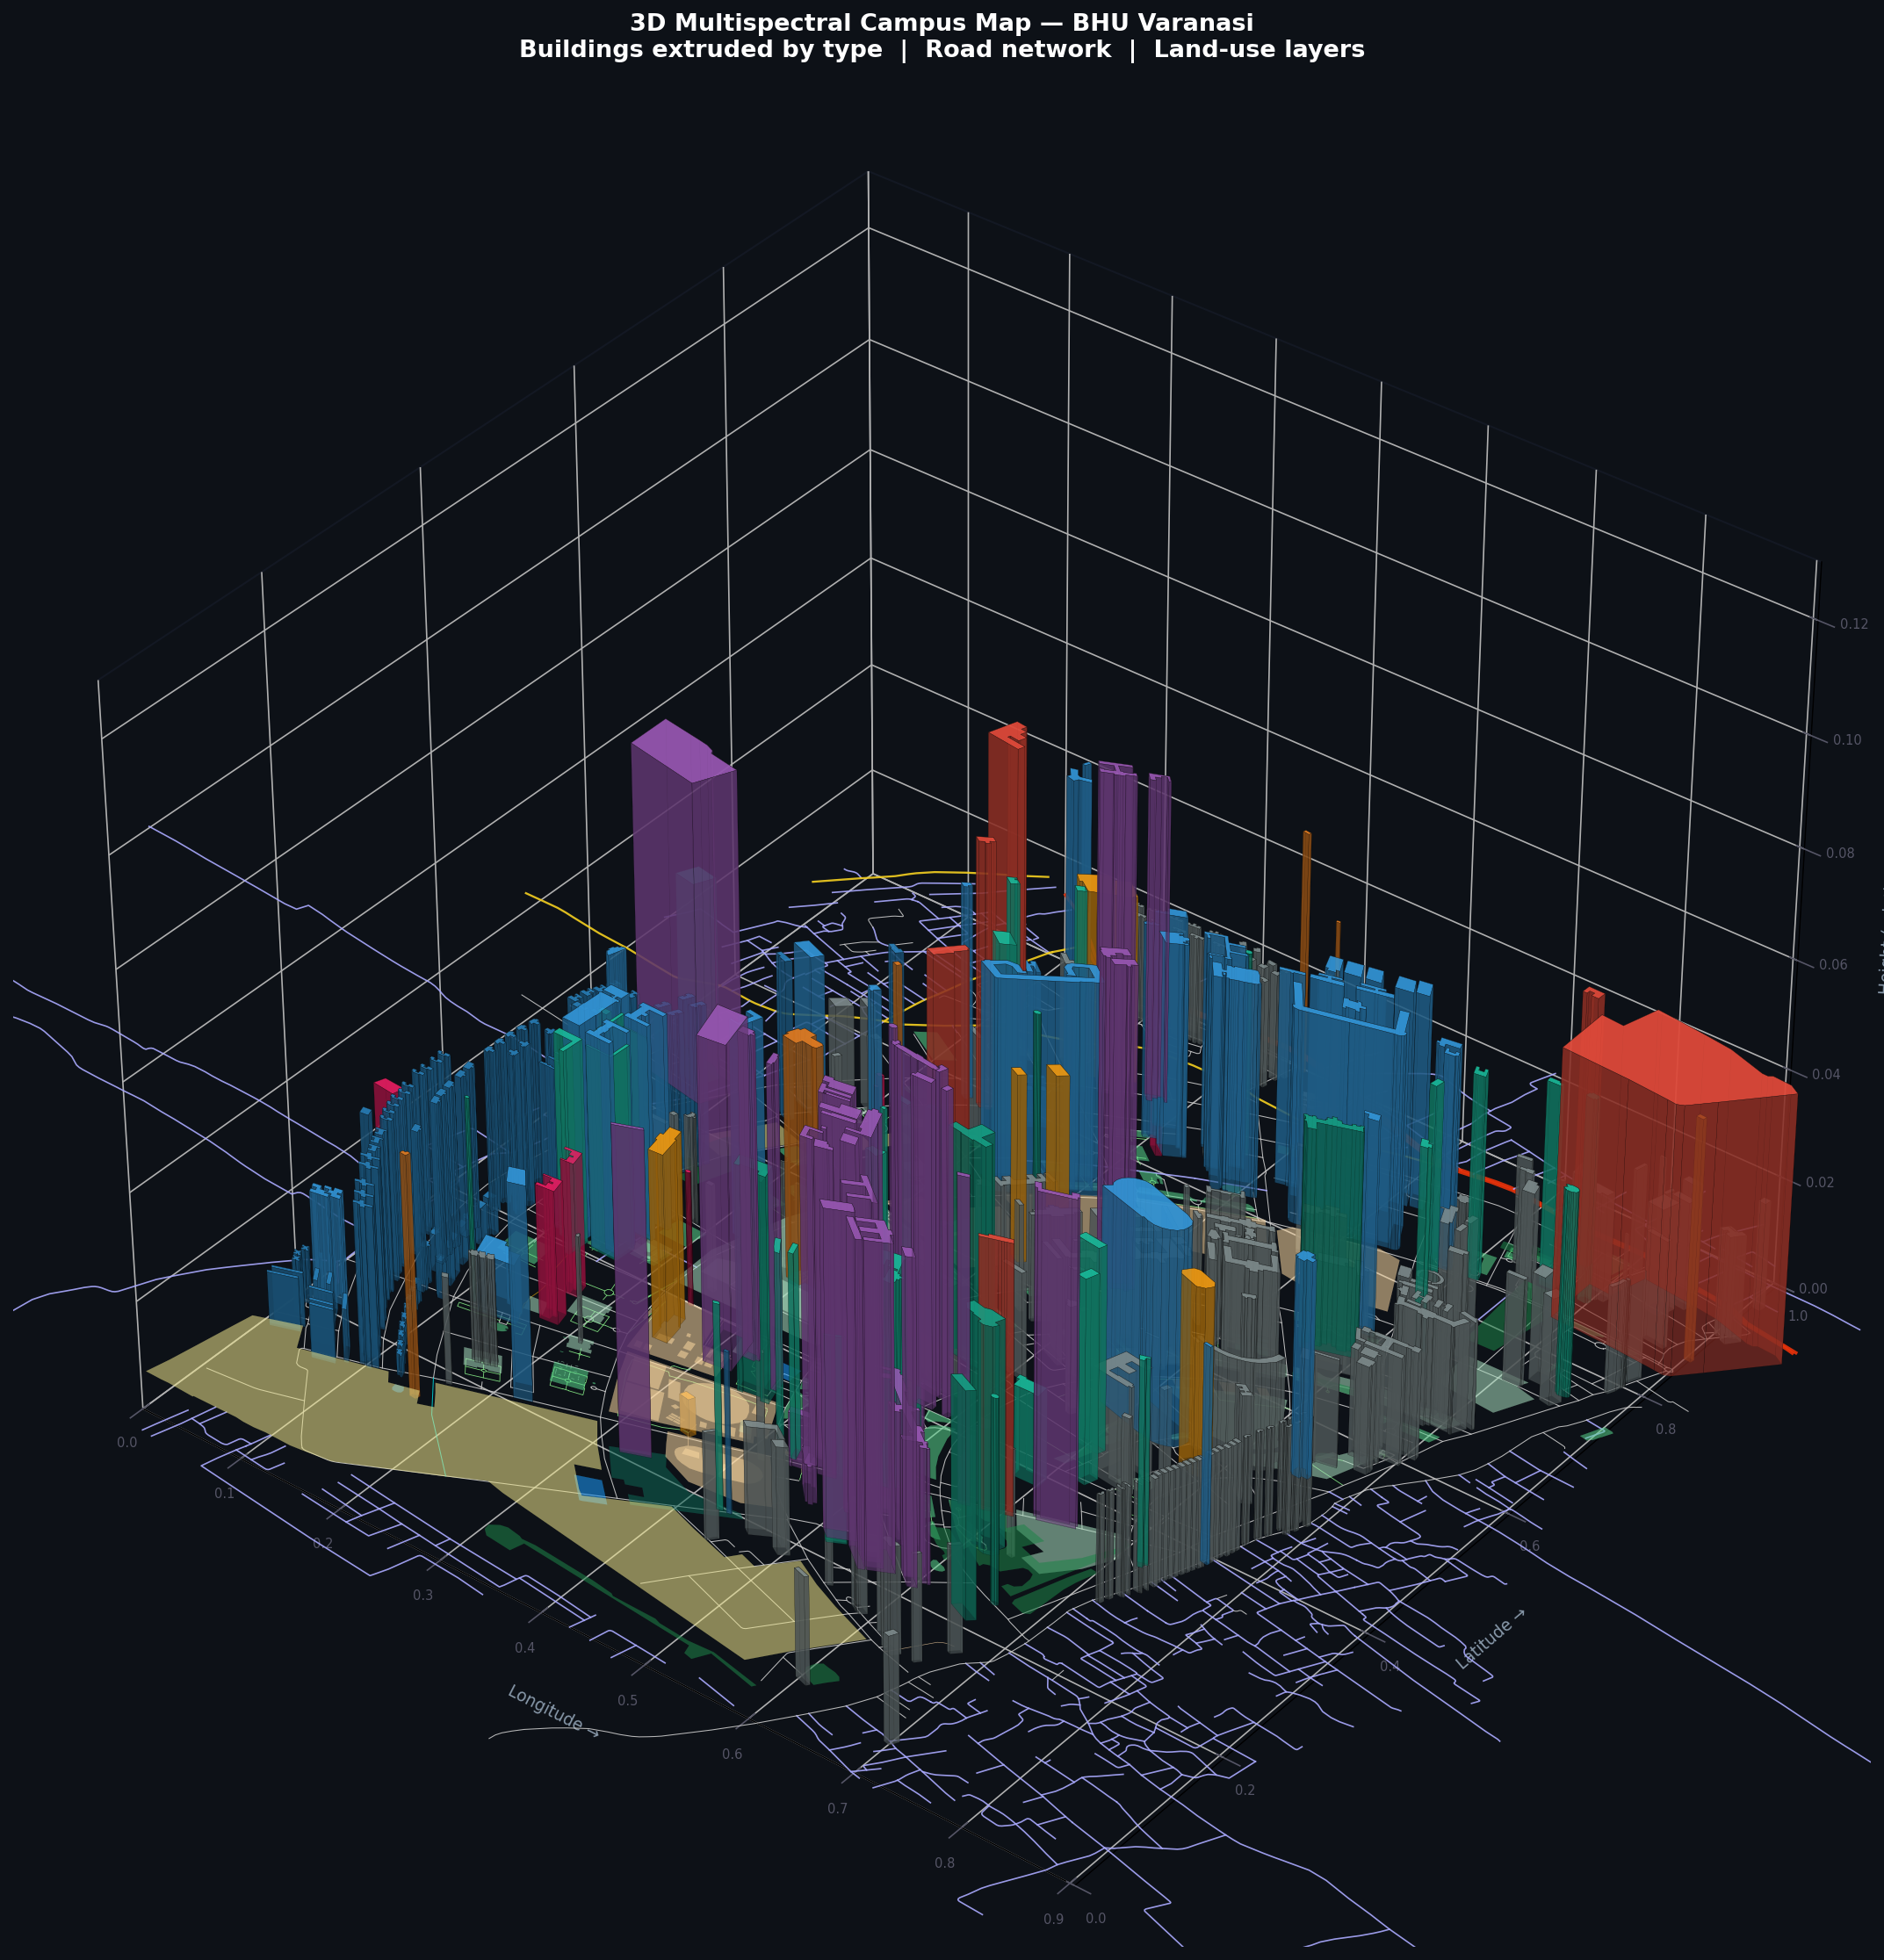
\includegraphics[width=0.45\textwidth]{figures/bhu_3d.png}}
\caption{3D Extruded Multispectral Map of BHU Campus. Buildings are extruded based on their functional category. Academic blocks (violet) are tallest; generic buildings (grey) are shortest.}
\label{fig:bhu_3d}
\end{figure}



\section{Phase 2: Machine Learning-Based EV Station Prediction}

\subsection{Motivation for ML}

While the heuristic scoring in Phase~1 provides reasonable results within a single map, it has inherent limitations. Feature weights are manually assigned, introducing subjective bias. The model cannot learn from real-world patterns of where EV stations are actually built. It does not generalise---each new criterion requires manual coding. Phase~2 addresses these limitations by training a supervised ML model on real, existing EV charging station locations across Indian cities, learning the spatial feature patterns that characterise successful station placements, and applying those learned patterns to predict suitability on any new, unseen map.

\subsection{Training Data Generation}

\subsubsection{Data Source}

The training data source is \texttt{ev-charging-stations-india.csv} (228\,KB), a dataset containing latitude/longitude coordinates of existing EV charging stations across India.

\subsubsection{Feature Extraction via Overpass API}

For each station, the pipeline: (1) queries the free Overpass API for all OSM elements (nodes, ways, relations) within a 500-metre radius of the station's coordinates; (2) extracts 23 spatial features from the returned elements; (3) labels the sample as positive (label = 1); (4) generates $k = 2$ negative samples by offsetting the coordinates by approximately 1.5\,km in random directions (areas unlikely to host a charging station) and querying their features; and (5) introduces a 2-second delay between API calls to respect rate limits.

Up to 150 stations are sampled across multiple cities for geographic diversity. The generated training data is cached to \texttt{output/training\_data.csv} (433 samples in our run) for reproducibility and fast iteration.

\subsection{Feature Engineering}
\label{sec:features}

Each sample (both positive and negative) is represented by a 23-dimensional feature vector. Table~\ref{tab:features} presents the complete feature set.

\begin{table}[htbp]
\caption{Complete Feature Vector (23 Features)}
\begin{center}
\begin{tabular}{|r|l|l|}
\hline
\textbf{\#} & \textbf{Feature Name} & \textbf{Description} \\
\hline
1 & \texttt{road\_primary} & Primary road present \\
\hline
2 & \texttt{road\_secondary} & Secondary road present \\
\hline
3 & \texttt{road\_tertiary} & Tertiary road present \\
\hline
4 & \texttt{road\_residential} & Residential road present \\
\hline
5 & \texttt{road\_service} & Service road present \\
\hline
6 & \texttt{road\_any} & Any road present \\
\hline
7 & \texttt{road\_count\_norm} & Normalised road count \\
\hline
8 & \texttt{parking\_nearby} & Parking amenity detected \\
\hline
9 & \texttt{amenity\_university} & University/college nearby \\
\hline
10 & \texttt{amenity\_hospital} & Hospital/clinic nearby \\
\hline
11 & \texttt{amenity\_rest\_cafe} & Restaurant/cafe nearby \\
\hline
12 & \texttt{amenity\_bank} & Bank/ATM nearby \\
\hline
13 & \texttt{amenity\_school} & School nearby \\
\hline
14 & \texttt{amenity\_conference} & Conference centre nearby \\
\hline
15 & \texttt{amenity\_any} & Normalised amenity count \\
\hline
16 & \texttt{landuse\_education} & Education land use \\
\hline
17 & \texttt{landuse\_commercial} & Commercial land use \\
\hline
18 & \texttt{landuse\_residential} & Residential land use \\
\hline
19 & \texttt{landuse\_recreation} & Recreation land use \\
\hline
20 & \texttt{building\_count} & Normalised building count \\
\hline
21 & \texttt{node\_density} & Normalised OSM node count \\
\hline
22 & \texttt{has\_existing\_ev} & Existing EV station tag \\
\hline
23 & \texttt{poi\_density} & Normalised POI count \\
\hline
\end{tabular}
\label{tab:features}
\end{center}
\end{table}

\subsection{Model Architecture}

A Random Forest Classifier is used with the hyperparameters shown in Table~\ref{tab:rf_params}. The \texttt{class\_weight='balanced'} option automatically adjusts weights inversely proportional to class frequencies, addressing the class imbalance inherent in the 1:2 positive-to-negative sampling ratio.

\begin{table}[htbp]
\caption{Random Forest Hyperparameters}
\begin{center}
\begin{tabular}{|l|l|}
\hline
\textbf{Parameter} & \textbf{Value} \\
\hline
Number of trees (\texttt{n\_estimators}) & 300 \\
\hline
Maximum depth (\texttt{max\_depth}) & 10 \\
\hline
Class weight balancing & \texttt{balanced} \\
\hline
Random state & 42 \\
\hline
Bootstrap sampling & True (default) \\
\hline
Split criterion & Gini impurity \\
\hline
\end{tabular}
\label{tab:rf_params}
\end{center}
\end{table}

\subsection{Training and Validation}

The model is evaluated using 5-fold Stratified Cross-Validation with ROC-AUC as the scoring metric, ensuring that class proportions are maintained across all folds. Table~\ref{tab:cv} presents the per-fold results.

\begin{table}[htbp]
\caption{Cross-Validation Results Per Fold}
\begin{center}
\begin{tabular}{|l|r|}
\hline
\textbf{Fold} & \textbf{ROC-AUC} \\
\hline
Fold 1 & 0.715 \\
\hline
Fold 2 & 0.638 \\
\hline
Fold 3 & 0.694 \\
\hline
Fold 4 & 0.586 \\
\hline
Fold 5 & 0.756 \\
\hline
\textbf{Mean} & \textbf{0.678} \\
\hline
\end{tabular}
\label{tab:cv}
\end{center}
\end{table}

A mean AUC of 0.678 indicates that the model performs meaningfully above random chance (0.5) at distinguishing suitable from unsuitable locations, though there is room for improvement with richer training data and additional features.

\begin{figure}[htbp]
\centerline{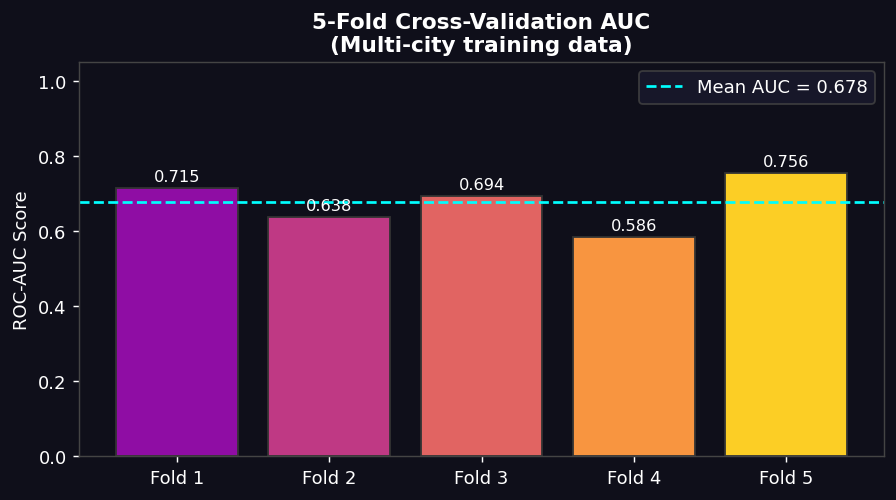
\includegraphics[width=0.45\textwidth]{figures/cv_auc.png}}
\caption{5-fold stratified cross-validation ROC-AUC scores. Mean AUC = 0.678 across all folds.}
\label{fig:cv_auc}
\end{figure}

\subsection{Feature Importance}

Feature importance is computed via Mean Decrease Impurity (MDI) from the trained Random Forest. Fig.~\ref{fig:feat_imp} shows the ranked importances.

\begin{figure}[htbp]
\centerline{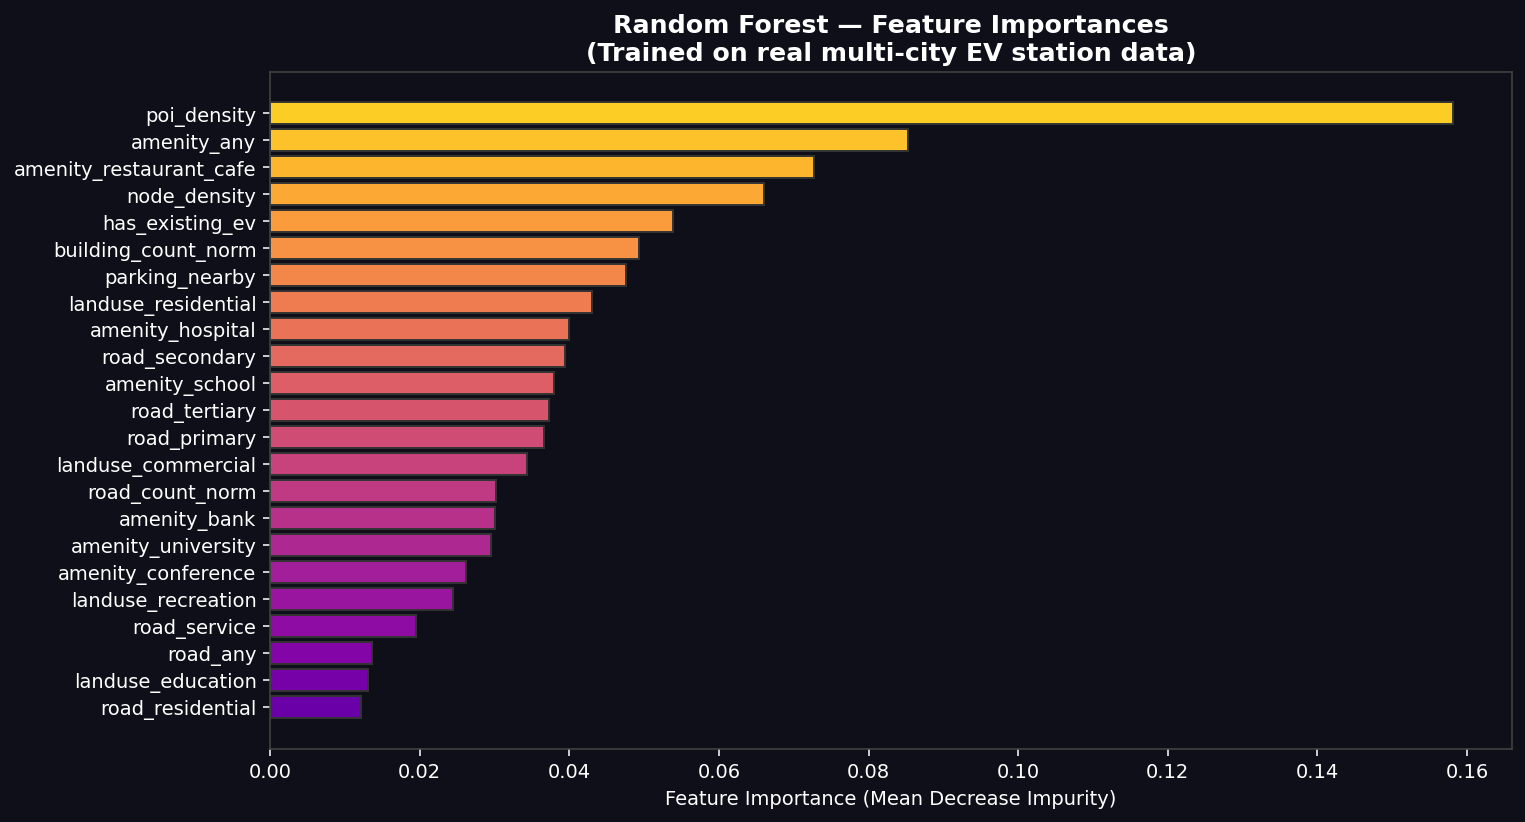
\includegraphics[width=0.48\textwidth]{figures/feature_importance.png}}
\caption{Random Forest feature importances ranked by Mean Decrease Impurity (MDI). POI density is the single most discriminative feature.}
\label{fig:feat_imp}
\end{figure}

Key findings from the feature importance analysis: (1) \texttt{poi\_density} (0.16) is the single most important feature---real EV stations are located in areas with high Point-of-Interest density; (2) \texttt{amenity\_any} (0.09) indicates general amenity count strongly distinguishes positive from negative samples; (3) \texttt{amenity\_restaurant\_cafe} (0.07) shows restaurants and cafes serve as proxies for foot traffic and dwell time; (4) \texttt{node\_density} (0.07) demonstrates raw OSM data density correlates with urban development intensity; and (5) \texttt{has\_existing\_ev} (0.06) confirms co-location of multiple chargers in the same zone is a strong signal.

\subsection{Prediction Pipeline}

Once the model is trained and saved as \texttt{ev\_model.joblib}, prediction on a new map proceeds as follows: (1) parse the \texttt{.osm} file to extract all nodes, ways, and the bounding box; (2) build a spatial index for efficient neighbour lookups; (3) divide the bounding box into a grid with approximately 111-metre cell resolution; (4) for each grid cell, extract the 23-feature vector by querying the spatial index for elements within a 330-metre radius; (5) feed the feature matrix to the trained Random Forest and obtain class probabilities $P(\text{suitable})$ for each cell; (6) deduplicate and rank the top candidates; and (7) generate output maps and JSON report. This prediction step is entirely offline and completes in under 10 seconds for typical campus-sized maps.


\section{Results and Case Studies}

\subsection{Case Study 1: BHU Campus, Varanasi}

BHU campus contains 15,162 nodes and 1,686 ways, including 915 road segments, 421 buildings, and 137 land-use polygons. Table~\ref{tab:bhu_heur} shows the heuristic results and Table~\ref{tab:bhu_ml} shows the ML results.

\begin{table}[htbp]
\caption{BHU Campus --- Heuristic Top EV Candidate Zones}
\begin{center}
\begin{tabular}{|r|l|c|}
\hline
\textbf{Rank} & \textbf{Location} & \textbf{Score} \\
\hline
1 & Swatantrata Bhavan & 0.47 \\
\hline
2 & Carpentry Workshop & 0.45 \\
\hline
3 & Main Library (IIT-BHU) & 0.45 \\
\hline
4 & Sir Sunderlal Hospital & 0.40 \\
\hline
5 & BHU DLW Road & 0.40 \\
\hline
\end{tabular}
\label{tab:bhu_heur}
\end{center}
\end{table}

\begin{table}[htbp]
\caption{BHU Campus --- ML-Predicted Top EV Candidate Zones}
\begin{center}
\begin{tabular}{|r|c|c|l|}
\hline
\textbf{Rank} & \textbf{Lat} & \textbf{Lon} & \textbf{Score / Tier} \\
\hline
1 & 25.2708 & 82.9820 & 0.586 / MEDIUM \\
\hline
2 & 25.2558 & 82.9870 & 0.579 / MEDIUM \\
\hline
3 & 25.2688 & 82.9940 & 0.569 / MEDIUM \\
\hline
4 & 25.2588 & 82.9850 & 0.564 / MEDIUM \\
\hline
5 & 25.2588 & 82.9930 & 0.561 / MEDIUM \\
\hline
\end{tabular}
\label{tab:bhu_ml}
\end{center}
\end{table}

The heuristic model identified 13 candidate zones, with Swatantrata Bhavan scoring highest due to its proximity to parking and the main road. The ML model found 7 unique candidate zones with scores ranging from 0.56 to 0.59, all classified as MEDIUM priority. The ML predictions corroborate several heuristic picks near the IIT campus core but also suggest zones in the southern residential area.

\begin{figure}[htbp]
\centerline{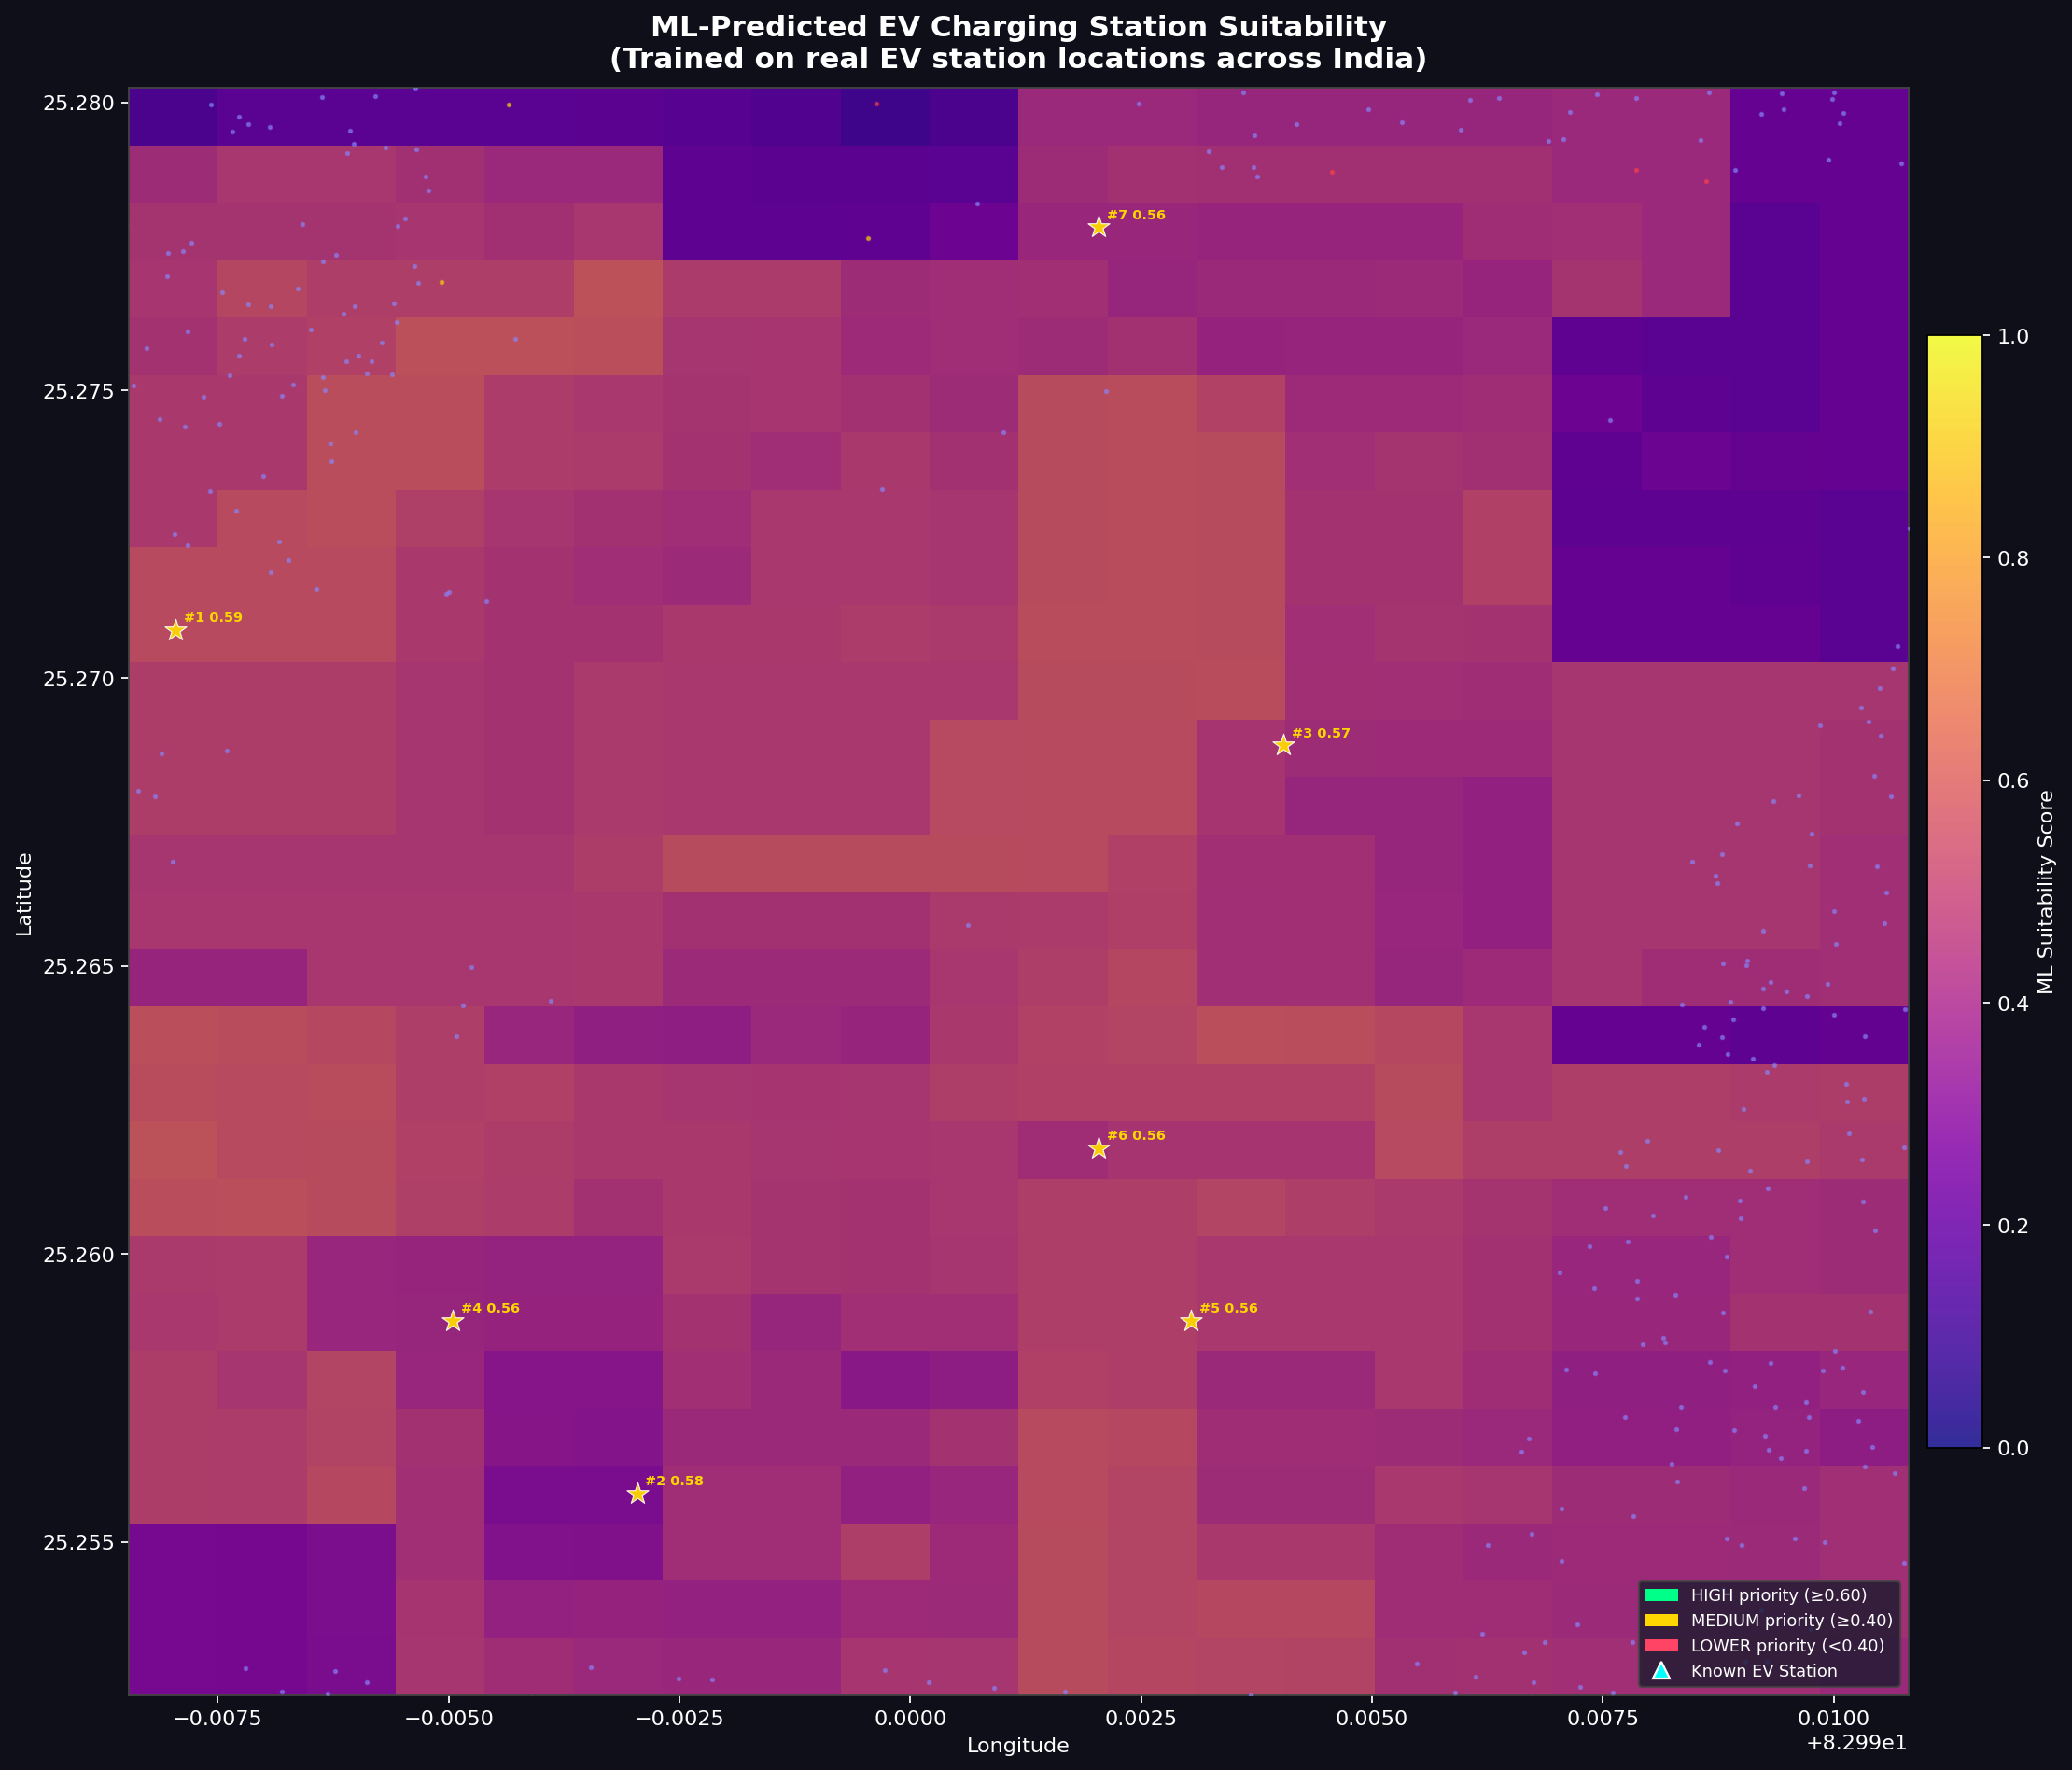
\includegraphics[width=0.45\textwidth]{figures/bhu_ml_prediction.png}}
\caption{ML-Predicted EV Charging Station Suitability for BHU Campus. Star markers show top-ranked candidate zones with ML scores.}
\label{fig:bhu_ml}
\end{figure}

\subsection{Case Study 2: IIT Delhi, New Delhi}

\begin{figure}[htbp]
\centerline{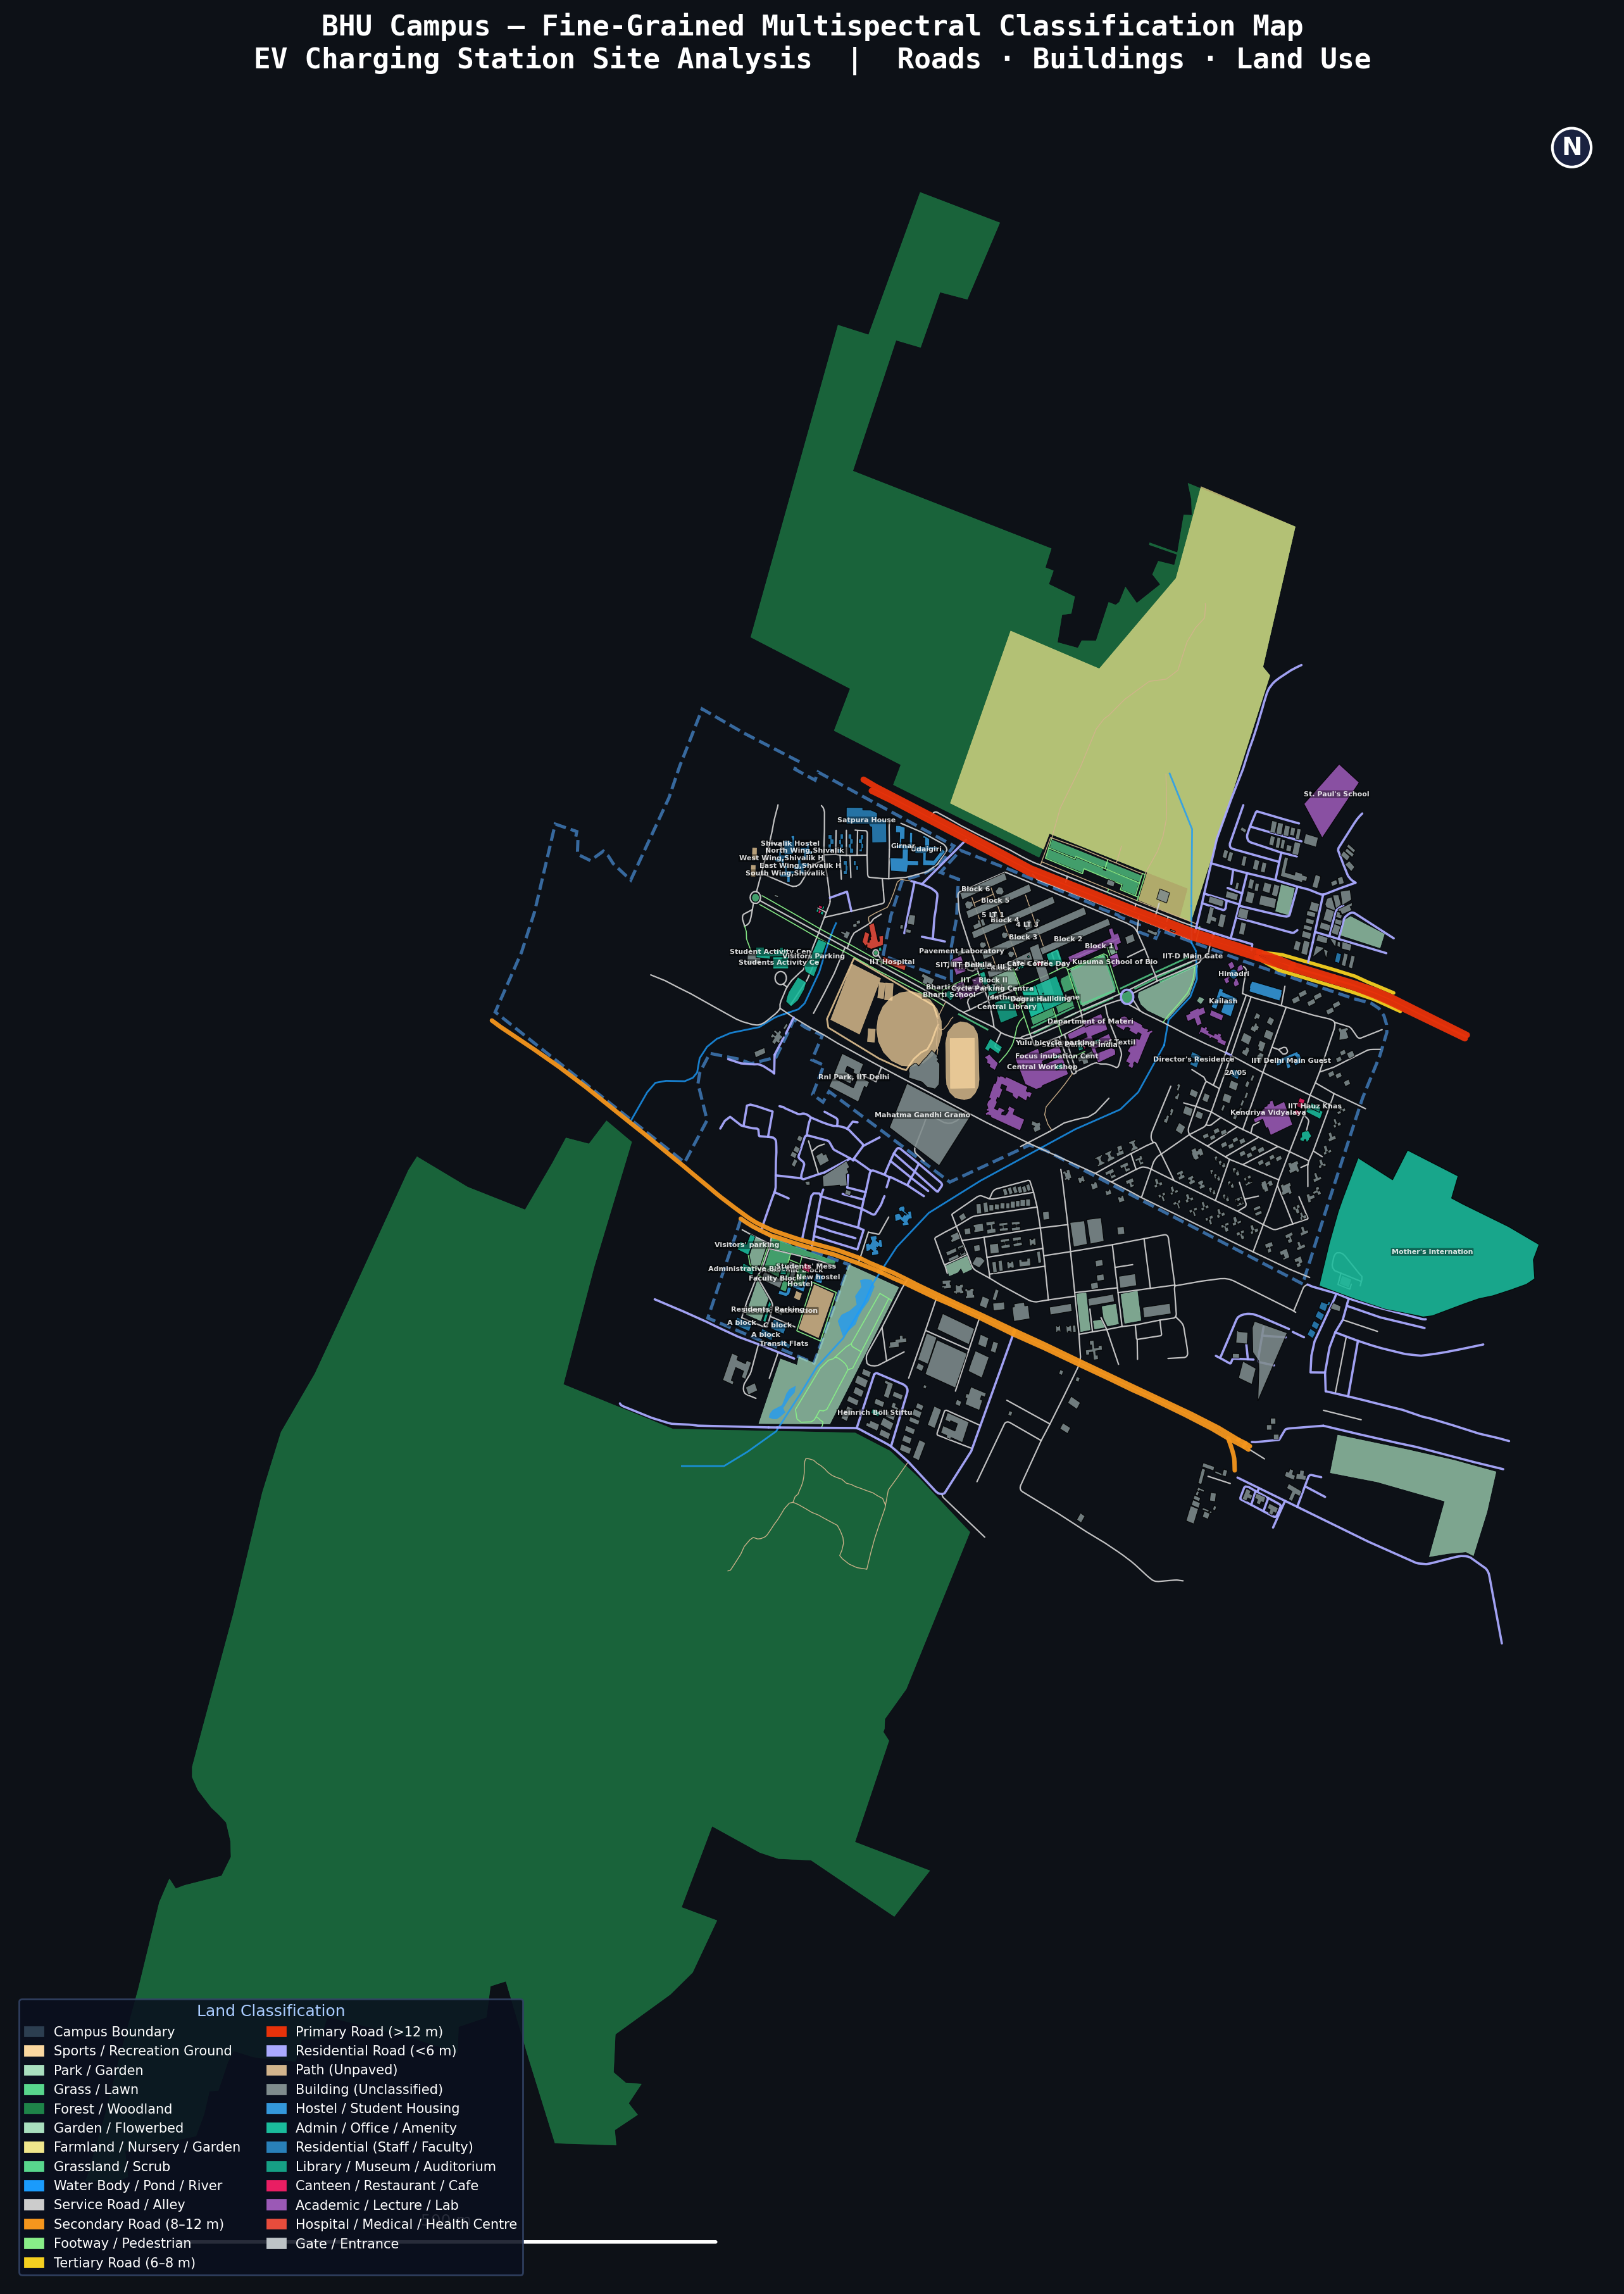
\includegraphics[width=0.45\textwidth]{figures/iitd_multispectral.png}}
\caption{Multispectral Classification Map for IIT Delhi Campus.}
\label{fig:iitd_multi}
\end{figure}

\begin{figure}[htbp]
\centerline{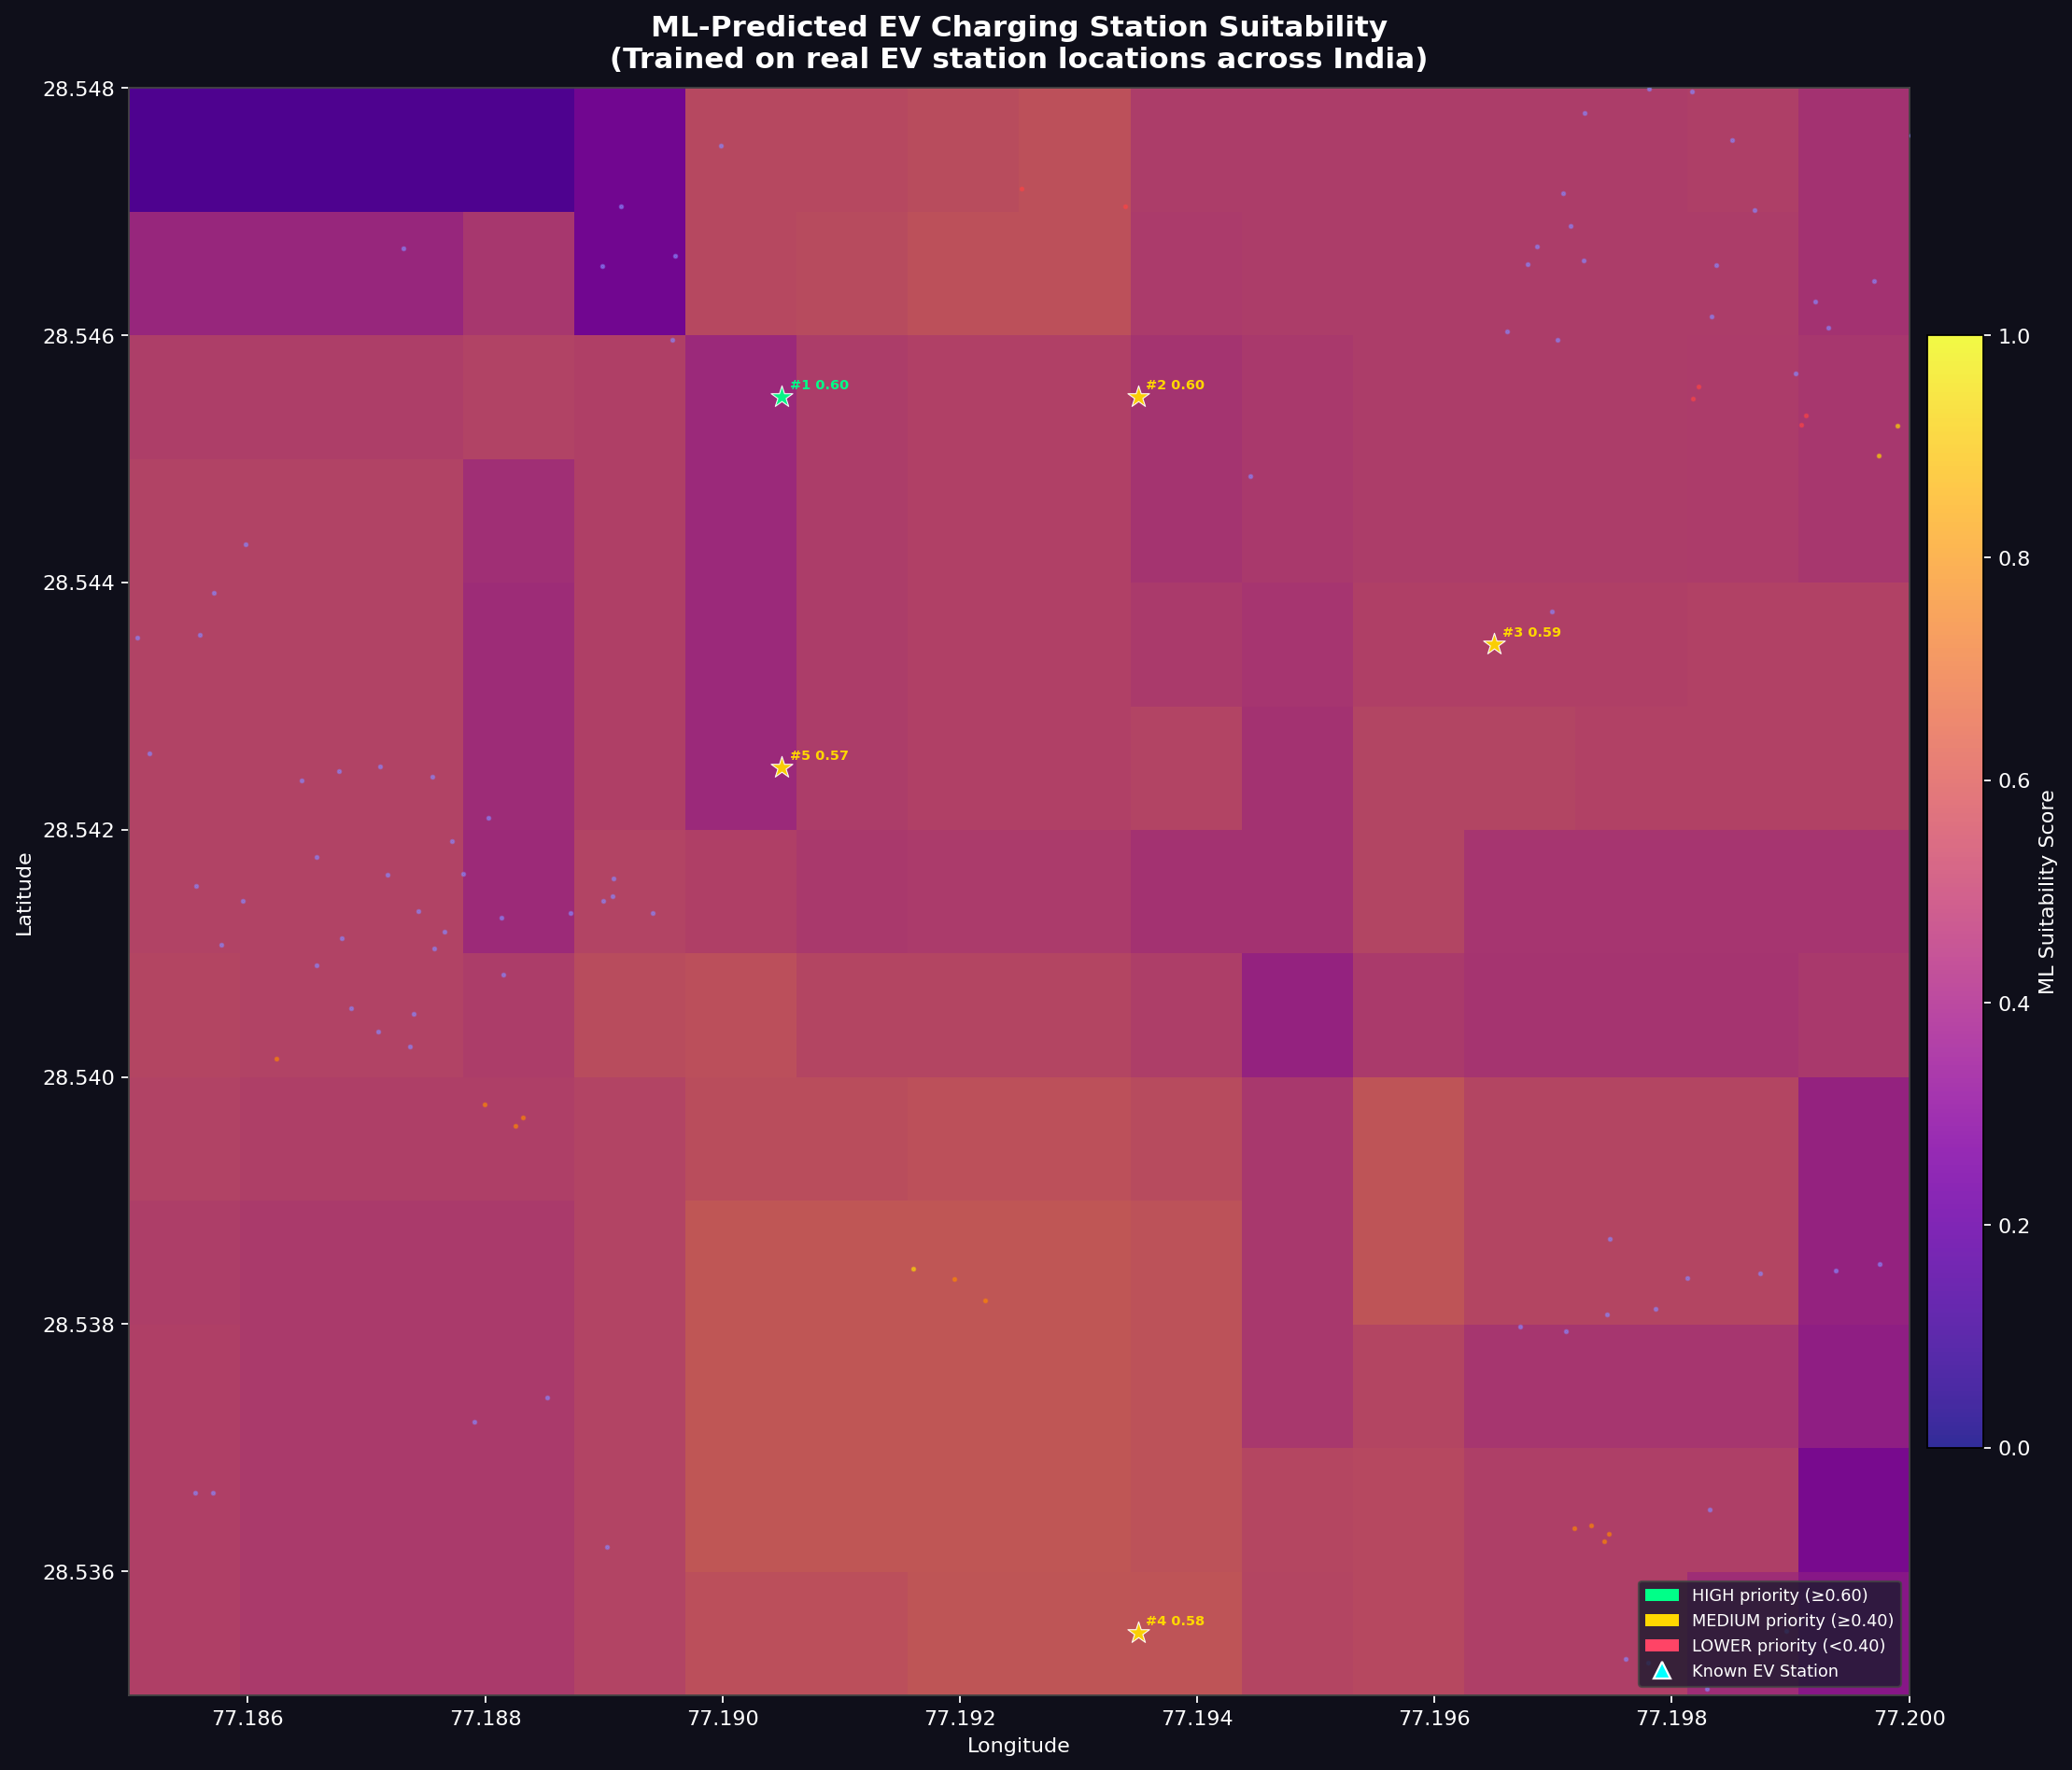
\includegraphics[width=0.45\textwidth]{figures/iitd_ml_prediction.png}}
\caption{ML Prediction Map for IIT Delhi Campus.}
\label{fig:iitd_ml}
\end{figure}

\begin{table}[htbp]
\caption{IIT Delhi --- ML-Predicted Top EV Candidate Zones}
\begin{center}
\begin{tabular}{|r|c|c|l|}
\hline
\textbf{Rank} & \textbf{Lat} & \textbf{Lon} & \textbf{Score / Tier} \\
\hline
1 & 28.5455 & 77.1905 & 0.600 / HIGH \\
\hline
2 & 28.5455 & 77.1935 & 0.598 / MEDIUM \\
\hline
3 & 28.5435 & 77.1965 & 0.592 / MEDIUM \\
\hline
4 & 28.5355 & 77.1935 & 0.577 / MEDIUM \\
\hline
5 & 28.5425 & 77.1905 & 0.572 / MEDIUM \\
\hline
\end{tabular}
\label{tab:iitd_ml}
\end{center}
\end{table}

The model's top candidate (score 0.6003) is rated HIGH priority---the only HIGH-priority result among the campus case studies. This location corresponds to the northern area of the IIT Delhi campus near the main gate and residential zones---a sensible placement for real-world EV charger deployment. The model successfully generalised from the training data (which included various Indian cities) to an entirely unseen campus in a different state.

\subsection{Case Study 3: Majestic Area, Bangalore}

\begin{figure}[htbp]
\centerline{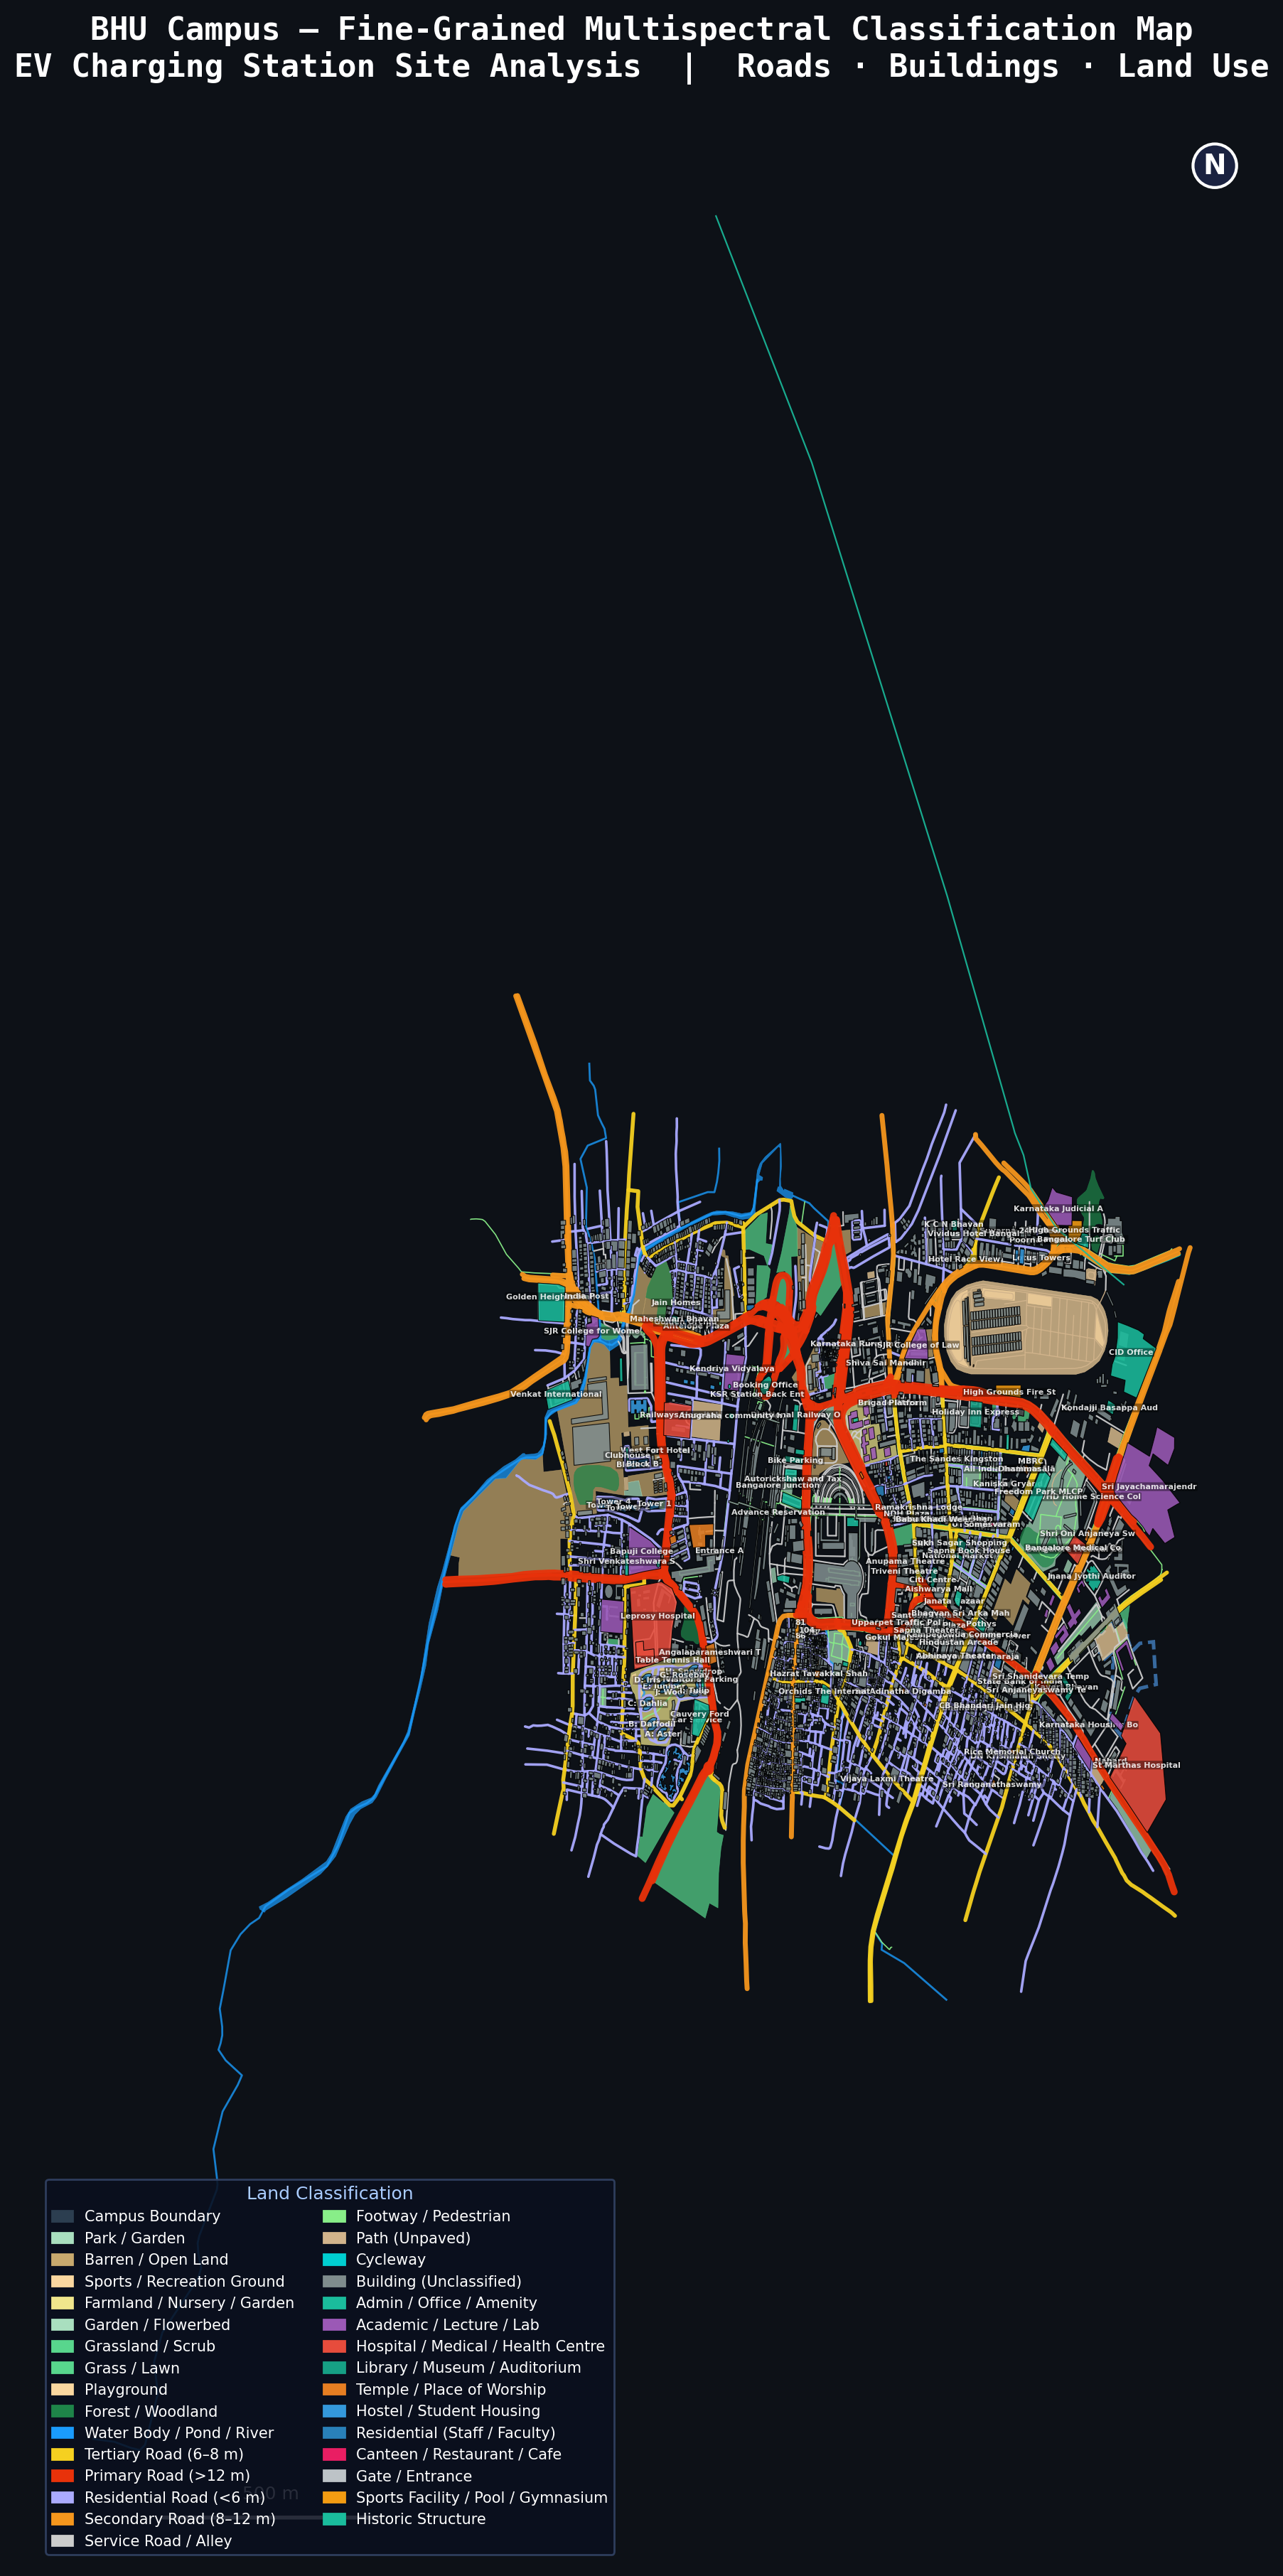
\includegraphics[width=0.45\textwidth]{figures/majestic_multispectral.png}}
\caption{Multispectral Classification Map for Bangalore Majestic Area.}
\label{fig:maj_multi}
\end{figure}

\begin{figure}[htbp]
\centerline{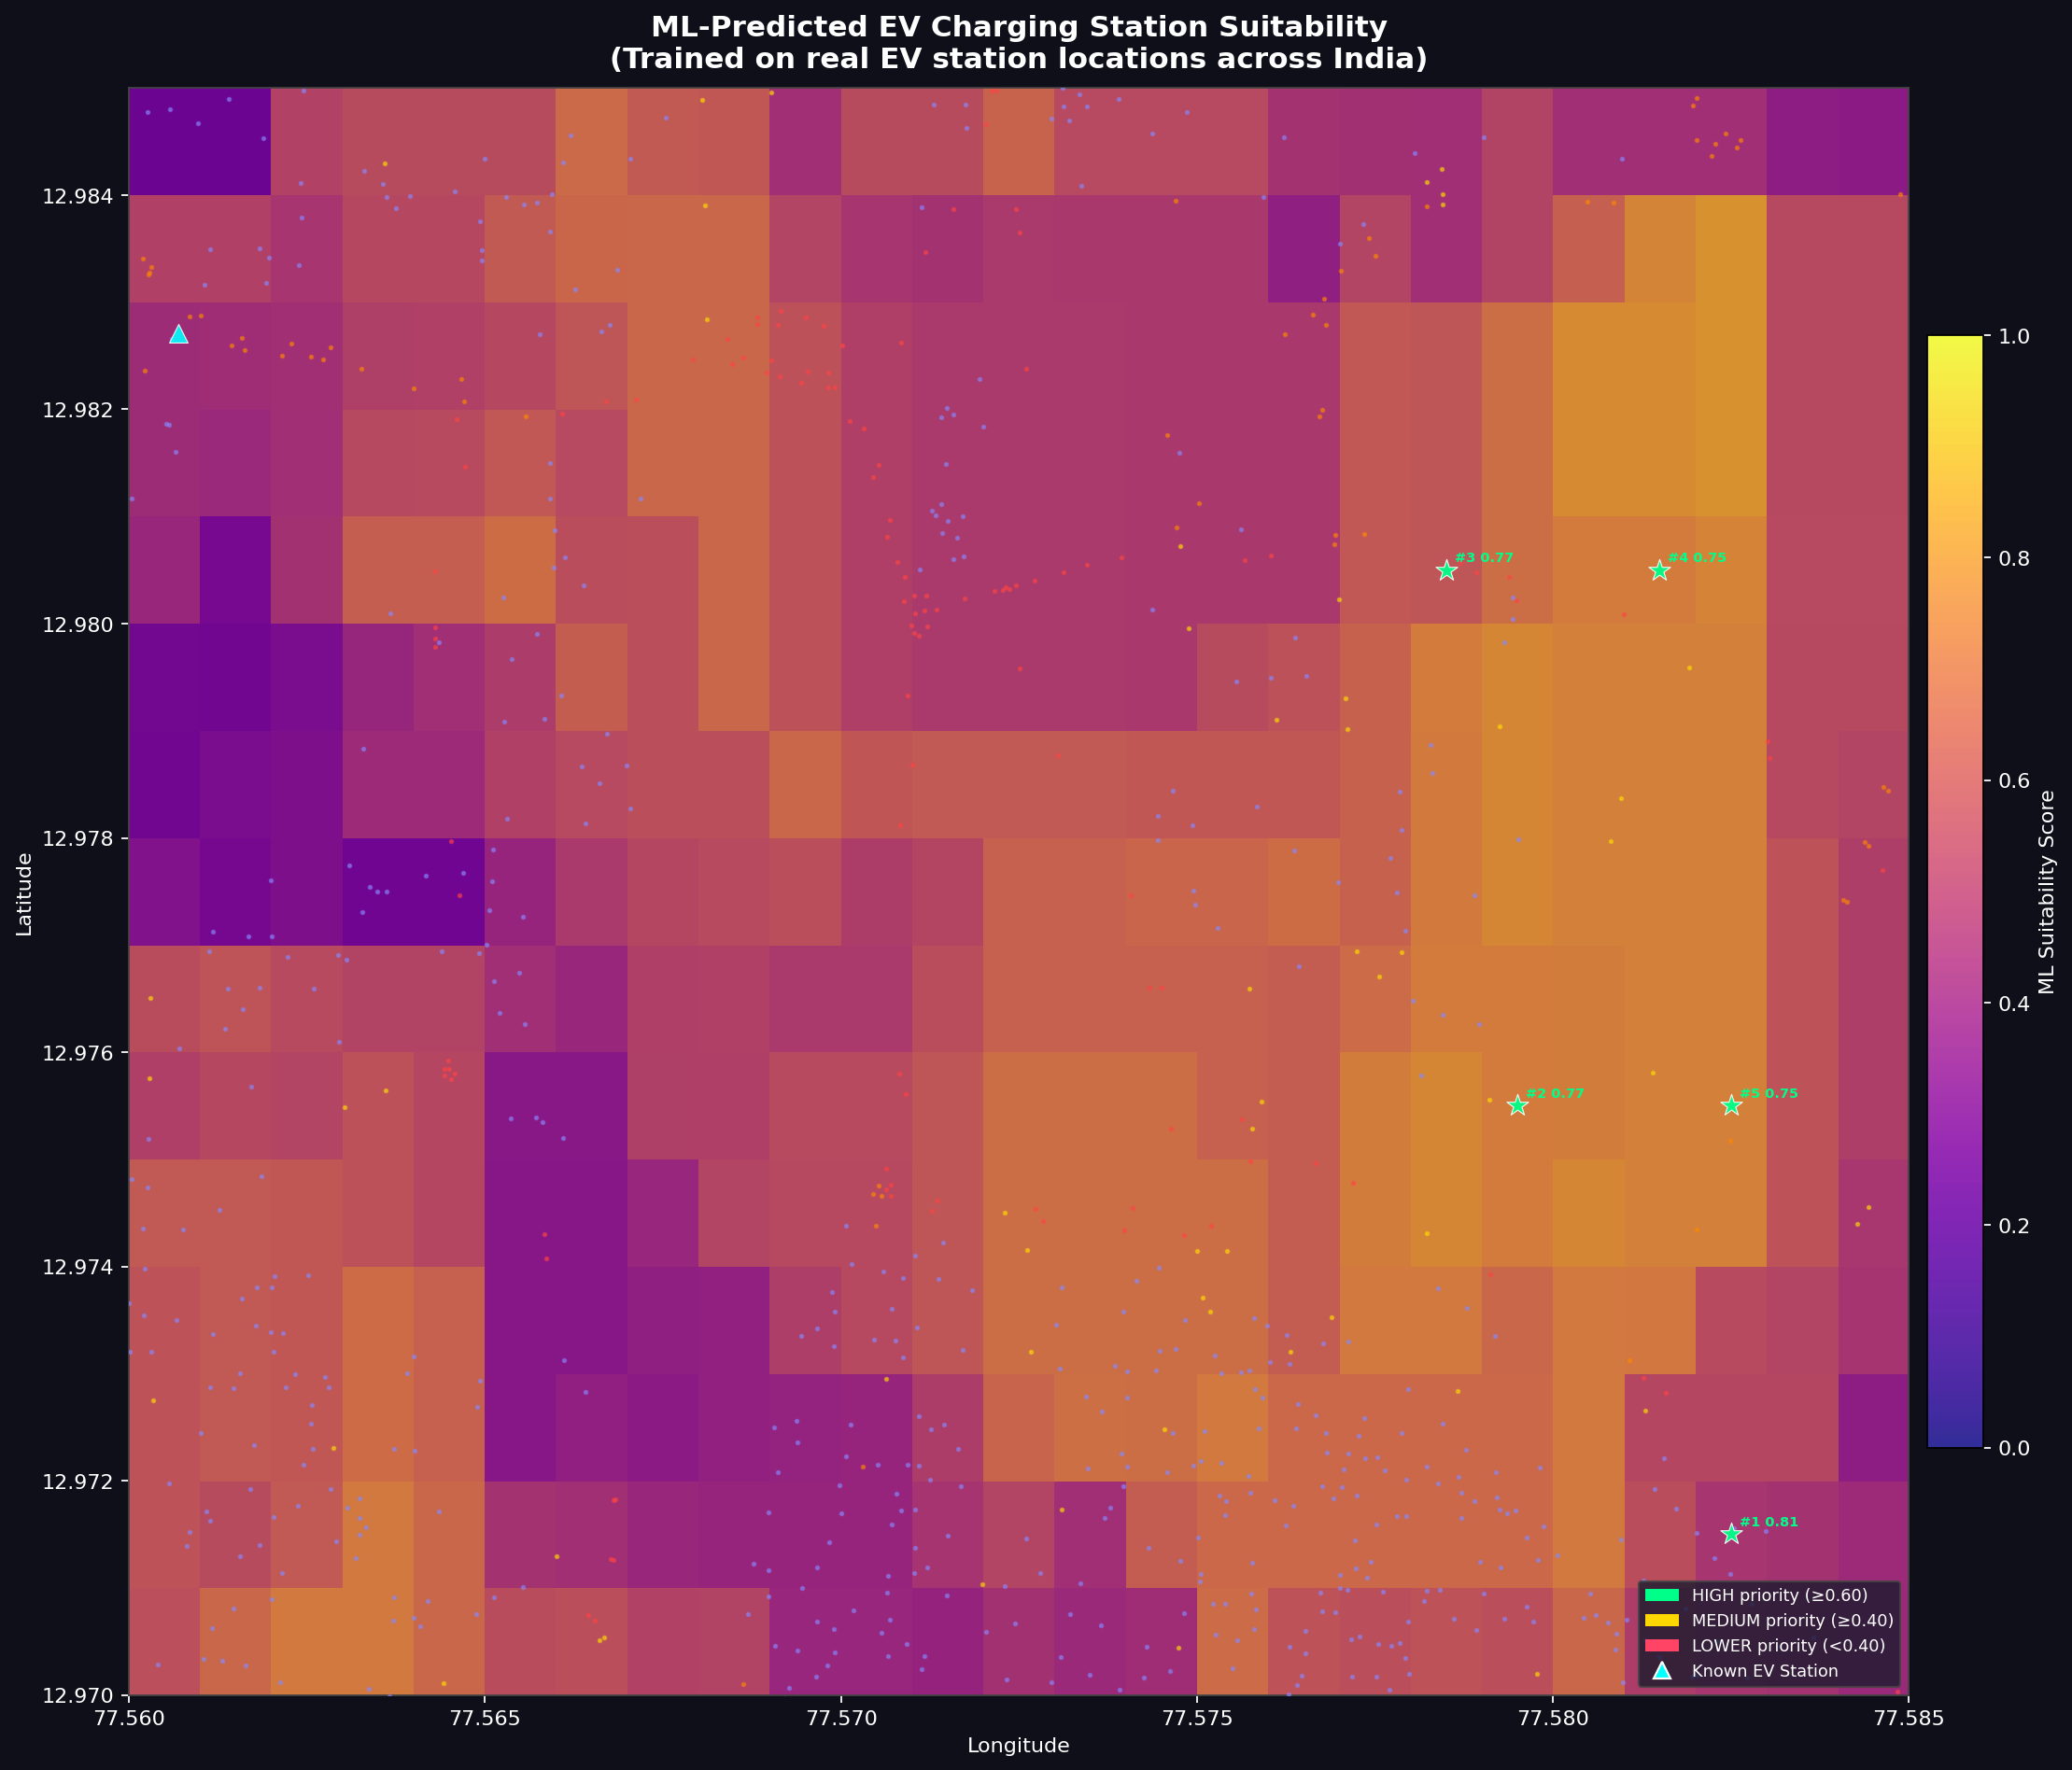
\includegraphics[width=0.45\textwidth]{figures/majestic_ml_prediction.png}}
\caption{ML Prediction Map for Bangalore Majestic Area.}
\label{fig:maj_ml}
\end{figure}

\begin{table}[htbp]
\caption{Bangalore Majestic --- ML-Predicted Top EV Candidate Zones}
\begin{center}
\begin{tabular}{|r|c|c|l|}
\hline
\textbf{Rank} & \textbf{Lat} & \textbf{Lon} & \textbf{Score / Tier} \\
\hline
1 & 12.9715 & 77.5825 & 0.811 / HIGH \\
\hline
2 & 12.9755 & 77.5795 & 0.772 / HIGH \\
\hline
3 & 12.9805 & 77.5785 & 0.772 / HIGH \\
\hline
4 & 12.9805 & 77.5815 & 0.754 / HIGH \\
\hline
5 & 12.9755 & 77.5825 & 0.751 / HIGH \\
\hline
\end{tabular}
\label{tab:majestic_ml}
\end{center}
\end{table}

All five top candidates are rated HIGH priority, with scores ranging from 0.75 to 0.81---significantly higher than the campus case studies. This aligns with expectations: Majestic is a dense commercial and transit hub with a major bus terminus, railway station, metro station, and extensive commercial activity. The model correctly identifies the high-density urban core as ideal for EV infrastructure---consistent with Bangalore's actual EV charging deployment patterns. The OSM file for Majestic was 9.0\,MB (compared to 3.4\,MB for BHU), reflecting much higher infrastructure density.

\subsection{Comparative Analysis}

\begin{table}[htbp]
\caption{Comparative Summary Across Three Test Sites}
\begin{center}
\begin{tabular}{|l|c|c|c|}
\hline
\textbf{Metric} & \textbf{BHU} & \textbf{IIT Delhi} & \textbf{Majestic} \\
\hline
OSM file size & 3.4\,MB & 1.9\,MB & 9.0\,MB \\
\hline
Area type & Campus & Campus & Urban \\
\hline
Total nodes & 15,162 & 8,441 & 42,637 \\
\hline
Total ways & 1,686 & 952 & 5,214 \\
\hline
Top ML score & 0.586 & 0.600 & 0.811 \\
\hline
HIGH-tier & 0 & 1 & 5 \\
\hline
MEDIUM-tier & 7 & 4 & 0 \\
\hline
Key zones & IIT core & Main gate & Transit hub \\
\hline
\end{tabular}
\label{tab:comp}
\end{center}
\end{table}

The comparative results demonstrate three key findings: (1) the model meaningfully differentiates between area types---dense urban zones score much higher than semi-rural campuses; (2) within campuses, the model favours areas near main roads, parking, and high-traffic amenities; and (3) the model generalises across geographies (Varanasi, Delhi, Bangalore) without retraining.


\section{Challenges and Limitations}

\subsection{Technical Challenges Encountered}

Several technical challenges were encountered during development:

\begin{enumerate}
\item \textbf{Non-numeric CSV data:} The EV station CSV contained latitude/longitude values stored as strings with embedded whitespace, causing \texttt{TypeError} during geometric calculations. This was fixed by applying \texttt{pd.to\_numeric()} with \texttt{errors='coerce'} and \texttt{dropna()}.

\item \textbf{Unicode encoding on Windows:} Progress indicators using UTF-8 checkmarks caused \texttt{UnicodeEncodeError} on Windows terminals using cp1252 encoding. Resolved by replacing Unicode symbols with ASCII equivalents.

\item \textbf{Overpass API rate limiting:} The free Overpass API imposes rate limits. Mitigated by adding 2-second delays between requests, implementing exponential backoff retries, and caching training data to disk.

\item \textbf{OSM data quality:} Many buildings in the BHU dataset are tagged only as \texttt{building=yes} with no functional information. This required extensive name-based keyword matching as a fallback classification strategy.
\end{enumerate}

\subsection{Limitations}

The current system has several limitations that should be acknowledged:

\begin{itemize}
\item \textbf{No satellite/remote sensing data:} Classification is purely from OSM vector tags, not actual multispectral imagery from satellites.

\item \textbf{No electrical grid data:} The model does not consider transformer capacity, substation proximity, or power grid constraints---critical factors for real-world charger deployment.

\item \textbf{No traffic data:} Real traffic volume counts are not available from OSM. Road hierarchy serves as an imperfect proxy.

\item \textbf{Model AUC = 0.678:} While above random chance, the model's discriminative power is moderate. This is likely due to feature limitations in OSM data and the noisy nature of the negative sample generation.

\item \textbf{No multipolygon support:} OSM relations (multipolygon buildings, complex boundaries) are not parsed; only simple way polygons are processed.

\item \textbf{Height data sparse:} Most buildings lack explicit \texttt{height=*} tags in OSM, so 3D heights are category-based defaults rather than actual measurements.
\end{itemize}


\section{Future Work}

Several directions for future improvement are identified:

\begin{enumerate}
\item \textbf{Enriched training data:} Incorporate global EV station datasets (OpenChargeMap API with 250,000+ locations worldwide) to significantly improve model AUC and geographic coverage.

\item \textbf{Feature augmentation:} Add population density (census data), traffic flow estimates (Google Roads API), electrical grid proximity (power infrastructure OSM tags), and elevation data to the feature vector.

\item \textbf{Advanced models:} Experiment with XGBoost, LightGBM, and spatial graph neural networks (GNNs) for improved spatial reasoning and higher prediction accuracy.

\item \textbf{Interactive web dashboard:} Build a Folium/Leaflet web map with interactive layers, filtering, and real-time Overpass queries for end-user accessibility.

\item \textbf{Real-time demand modelling:} Integrate EV registration data and ride-hailing patterns to model time-varying charging demand across different hours and seasons.

\item \textbf{Multi-objective optimisation:} Formulate station placement as a facility location problem minimising total travel distance while maximising coverage equity across underserved areas.

\item \textbf{Satellite image fusion:} Combine OSM features with actual multispectral satellite imagery (Sentinel-2) for true remote-sensing-based land use analysis and verification.
\end{enumerate}


\section{Reproducibility and Usage}

The entire pipeline is designed for easy reproducibility. Installation requires creating a Python virtual environment and installing dependencies via \texttt{pip install -r requirements.txt}. The full pipeline (classification + ML prediction) is executed via \texttt{python main.py --osm map.osm --output ./output}. Training mode (one-time, requires internet) is invoked with \texttt{python main.py --train --csv ev-charging-stations-india.csv}. Prediction on any new area requires only an OSM file: \texttt{python main.py --osm new\_area.osm --output ./output\_new}. OSM data for any area in the world can be downloaded from openstreetmap.org or via the Overpass API.


\section{Conclusion}

This paper presents an end-to-end, open-data-driven approach to identifying optimal Electric Vehicle charging station locations. By combining a multispectral classification engine that translates raw OSM tags into rich, colour-coded spatial maps, a heuristic scoring model that ranks zones based on domain knowledge of EV infrastructure requirements, and a supervised Random Forest classifier trained on real EV station coordinates from across India, the system provides actionable, spatially-explicit recommendations for EV charger deployment on any geographic area available in OpenStreetMap---without requiring proprietary software, GIS licenses, or satellite imagery.

The pipeline was validated on three diverse sites: a large university campus (BHU), a compact technical institute (IIT Delhi), and a dense urban commercial zone (Bangalore Majestic). Results demonstrate that the model correctly identifies high-traffic urban zones (Majestic: all 5 candidates rated HIGH, scores 0.75--0.81) while assigning moderate scores to less urbanised campuses. Feature importance analysis reveals that POI density, amenity count, and restaurant/cafe presence are the strongest predictors---aligning with real-world station placement logic. The system generalises across Indian cities without retraining.

The entire codebase is open-source, lightweight (approximately 1,800 lines of Python), and runs on any machine with Python 3.8+ and standard ML libraries---no GPU required. The modular architecture allows easy extension with new data sources, ML models, and visualisation outputs.

\section*{Acknowledgment}

The authors acknowledge the OpenStreetMap community for maintaining the geospatial data used in this study, and the developers of scikit-learn~\cite{b4}, Matplotlib~\cite{b8}, and the Overpass API for providing open-source tools that made this work possible.

\begin{thebibliography}{00}
\bibitem{b1} NITI Aayog, Government of India, ``Electric vehicle charging infrastructure --- handbook for urban planners,'' 2022.
\bibitem{b2} OpenStreetMap Contributors, ``OpenStreetMap,'' Available: https://www.openstreetmap.org. [Accessed: Apr. 2026].
\bibitem{b3} Overpass API, ``Overpass API --- query language for OpenStreetMap,'' Available: https://wiki.openstreetmap.org/wiki/Overpass\_API. [Accessed: Mar. 2026].
\bibitem{b4} F. Pedregosa \textit{et al.}, ``Scikit-learn: machine learning in Python,'' \textit{J. Mach. Learn. Res.}, vol. 12, pp. 2825--2830, 2011.
\bibitem{b5} L. Breiman, ``Random forests,'' \textit{Mach. Learn.}, vol. 45, no. 1, pp. 5--32, 2001.
\bibitem{b6} Ministry of Heavy Industries, Government of India, ``FAME India scheme phase II,'' 2019. Available: https://fame2.heavyindustries.gov.in/.
\bibitem{b7} M. Kuby and S. Lim, ``The flow-refueling location model for alternative-fuel vehicles,'' \textit{Socio-Econ. Plan. Sci.}, vol. 39, no. 2, pp. 125--145, 2005.
\bibitem{b8} J. D. Hunter, ``Matplotlib: a 2D graphics environment,'' \textit{Comput. Sci. Eng.}, vol. 9, no. 3, pp. 90--95, 2007.
\end{thebibliography}

\end{document}
